\chapter{User Interface Design}
	While in the RASD we defined platform's proper UI structure, in this section we formalize navigation maps and present mock-up for each page:
	\begin{itemize}
		\item public pages:
		\begin{itemize}
			\item registration pages:
			\begin{itemize}
				\item \textbf{WelcomePage}
				\item \textbf{RegistrationMenuPage}
				\item \textbf{StudentRegistrationPage}
				\item \textbf{CompanyRegistrationPage}
			\end{itemize}
			\item logic pages:
			\begin{itemize}
				\item \textbf{LoginPage}
			\end{itemize}
		\end{itemize}
		\item private pages:
		\begin{itemize}
			\item profile pages:
			\begin{itemize}
				\item \textbf{StudentProfilePage}
				\item \textbf{CompanyProfilePage}
			\end{itemize}
			\item notifications pages:
			\begin{itemize}
				\item \textbf{NotificationsPage}
			\end{itemize}
			\item companies pages:
			\begin{itemize}
				\item \textbf{CompanySearchPage}
			\end{itemize}
			\item advice-related pages:
			\begin{itemize}
				\item \textbf{AdviceSearchPage}
				\item \textbf{PersonalAdvicePage}
				\item \textbf{PublishAdvicePage}
				\item \textbf{AdviceDetailsPage}
				\item \textbf{InterestingAdvicePage}
			\end{itemize}
			\item invites pages:
			\begin{itemize}
				\item \textbf{InvitesPage}
			\end{itemize}
			\item applications pages:
			\begin{itemize}
				\item \textbf{ApplicationsPage}
			\end{itemize}
			\item process-related pages:
			\begin{itemize}
				\item \textbf{ConfigProcessPage}
				\item \textbf{ProcessManagementPage}
				\item \textbf{StepsManagementPage}
				\item \textbf{ViewStatsPage}
				\item \textbf{ProcessFinalizationPage}
			\end{itemize}
			\item interviews pages:
			\begin{itemize}
				\item \textbf{InterviewsPage}
			\end{itemize}
			\item internships pages:
			\begin{itemize}
				\item \textbf{InternshipsPage}
				\item \textbf{InternshipDetailsPage}
			\end{itemize}
		\end{itemize}
	\end{itemize}
	
	Moreover, in this chapter we also specified how the sections defined in the User Interfaces section of the RASD are mapped onto the sections effectively designed.
	
	\section{Public pages}
	\subsection{Public pages navigation map}
	\begin{figure}[H]
		\centering
		\caption{Public pages navigation map}
		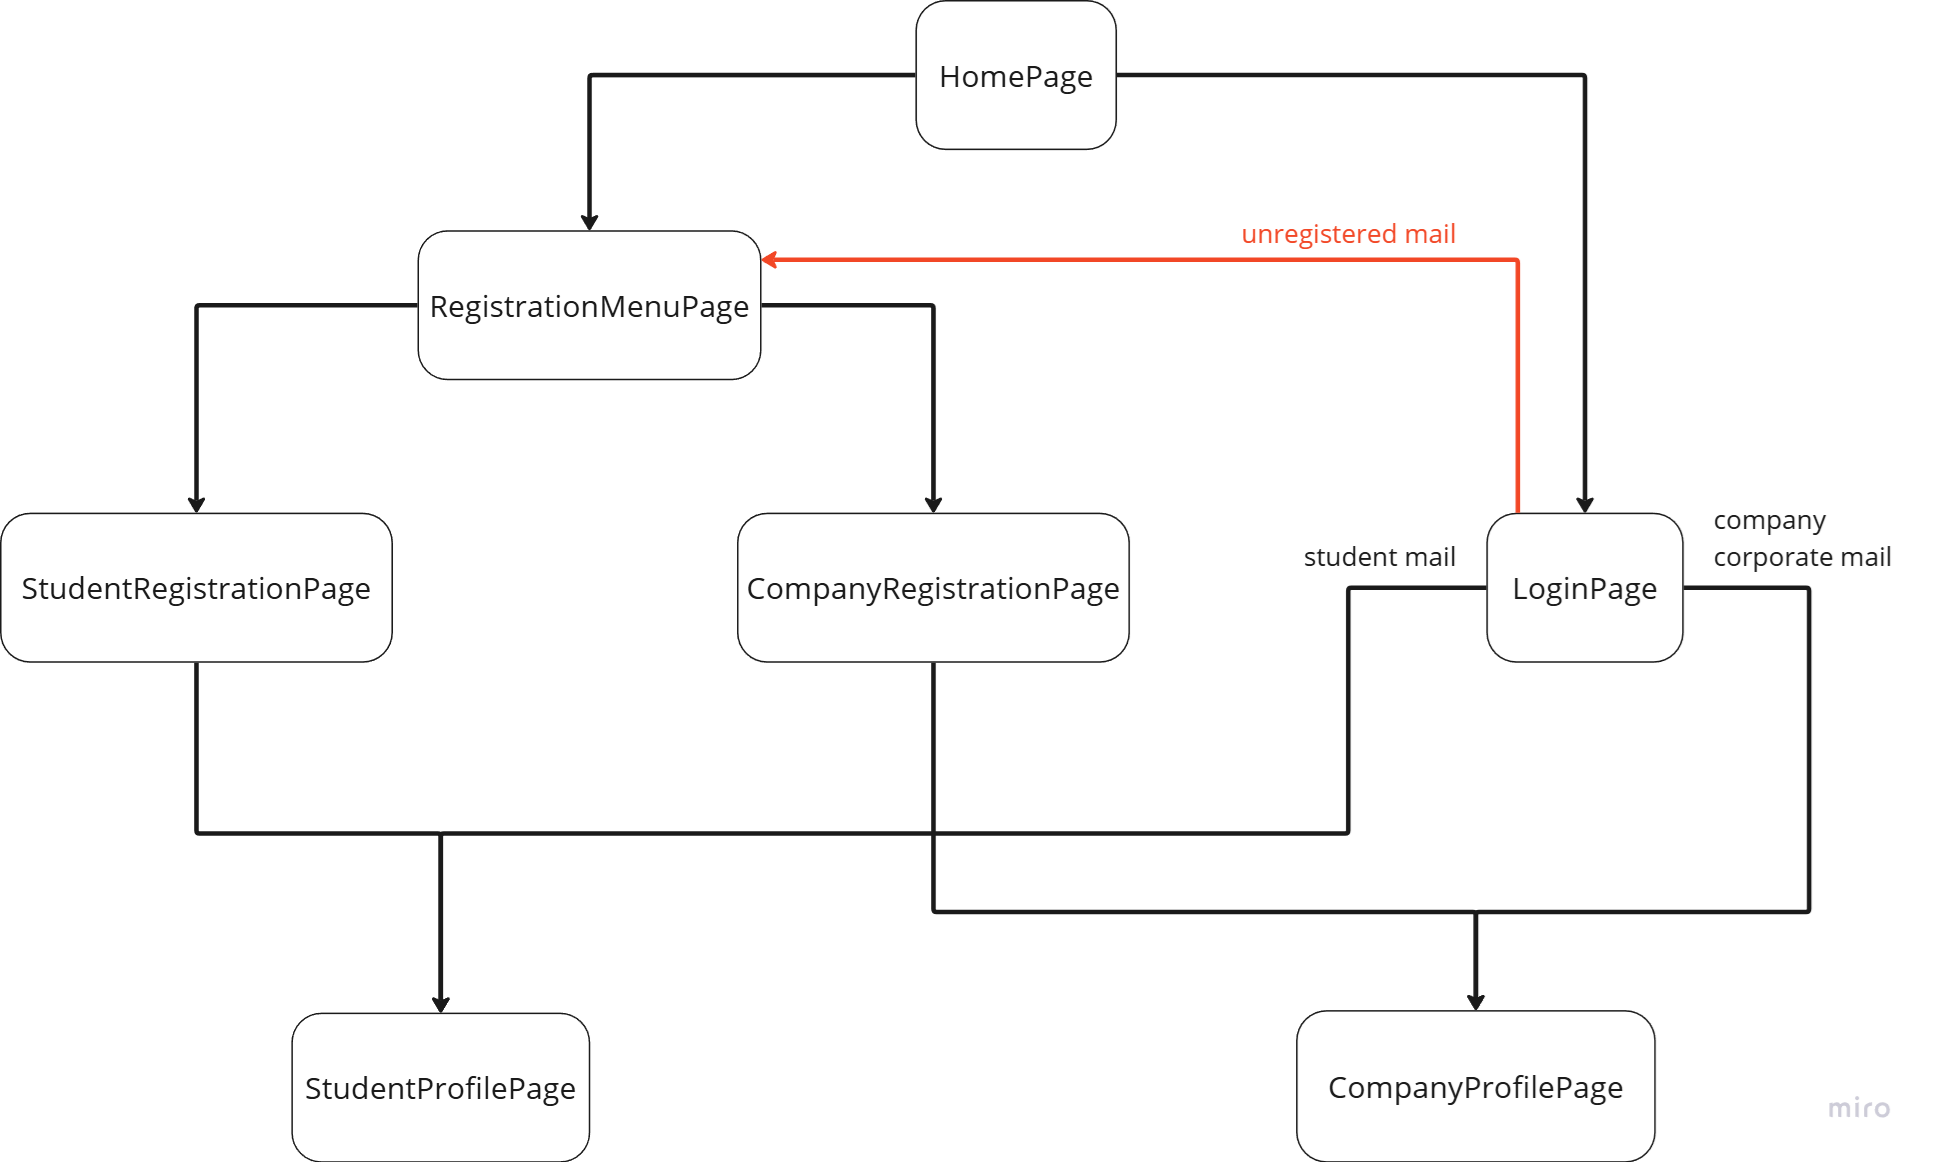
\includegraphics[width=13cm]{UI/publicMap.png}
	\end{figure}
	\subsection{Registration pages mock-up}
	\begin{figure}[H]
		\centering
		\caption{WelcomePage and RegistrationMenuPage mock-up}
		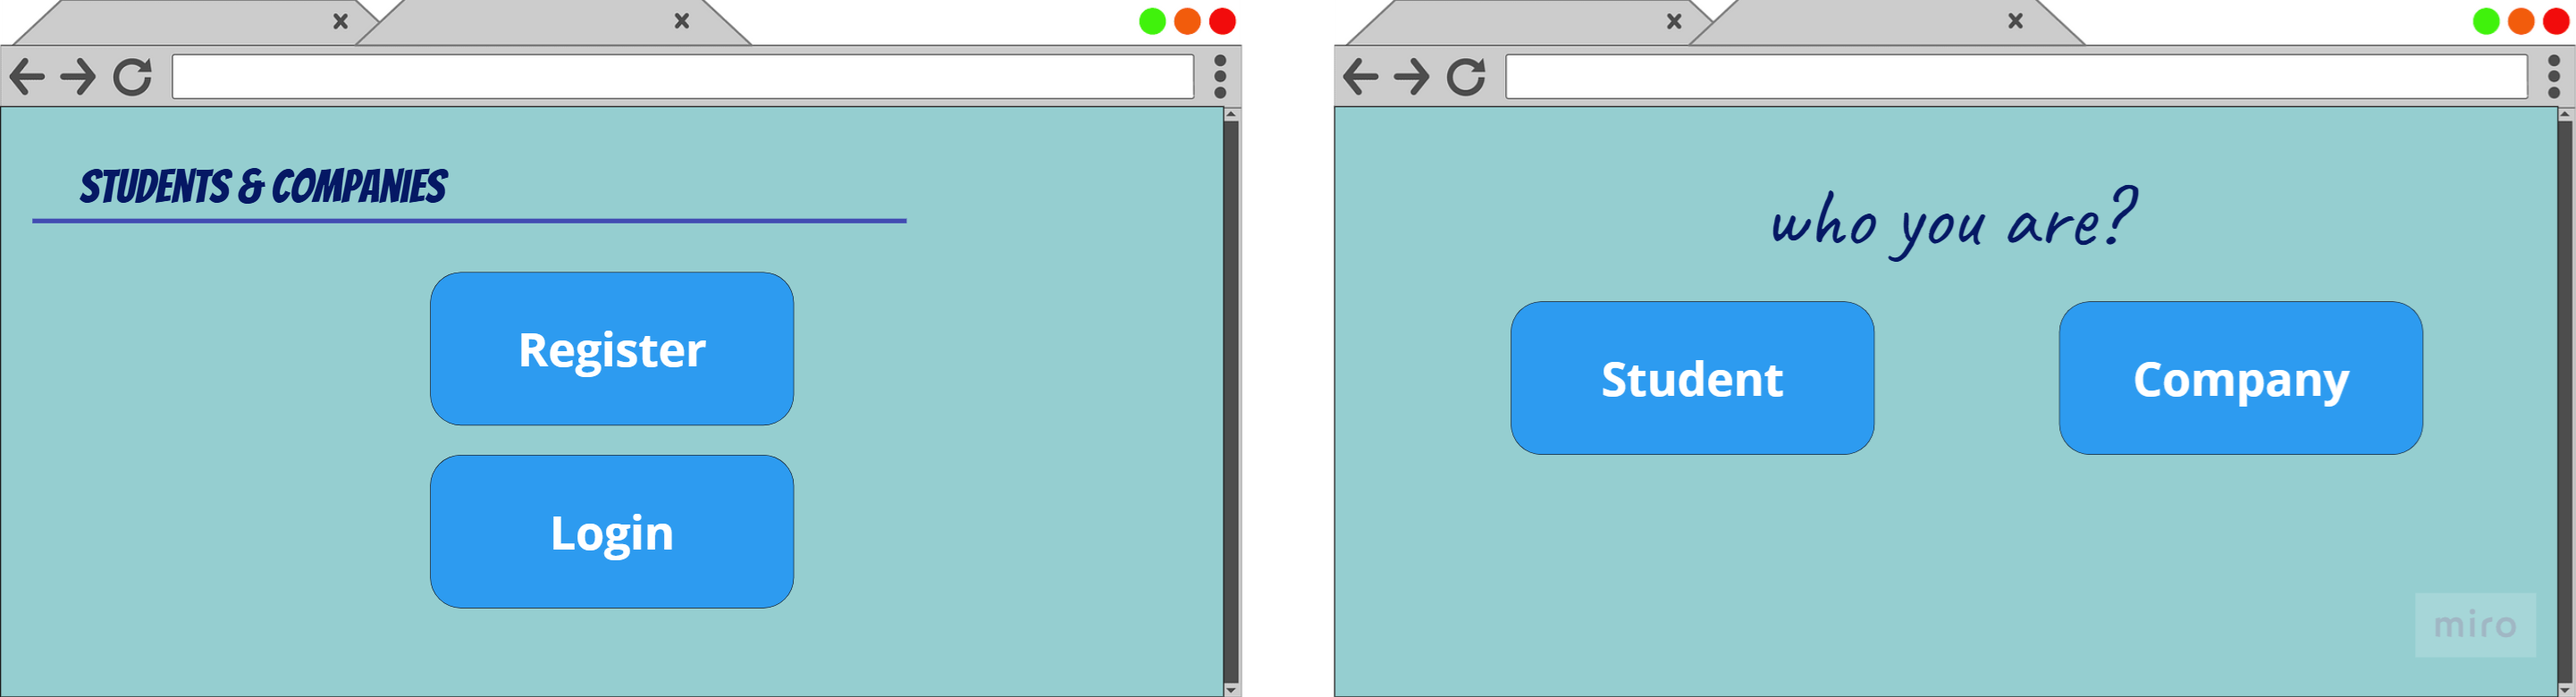
\includegraphics{UI/regIntro.png}
	\end{figure}
	\begin{figure}[H]
		\centering
		\caption{StudentRegistrationPage mock-up}
		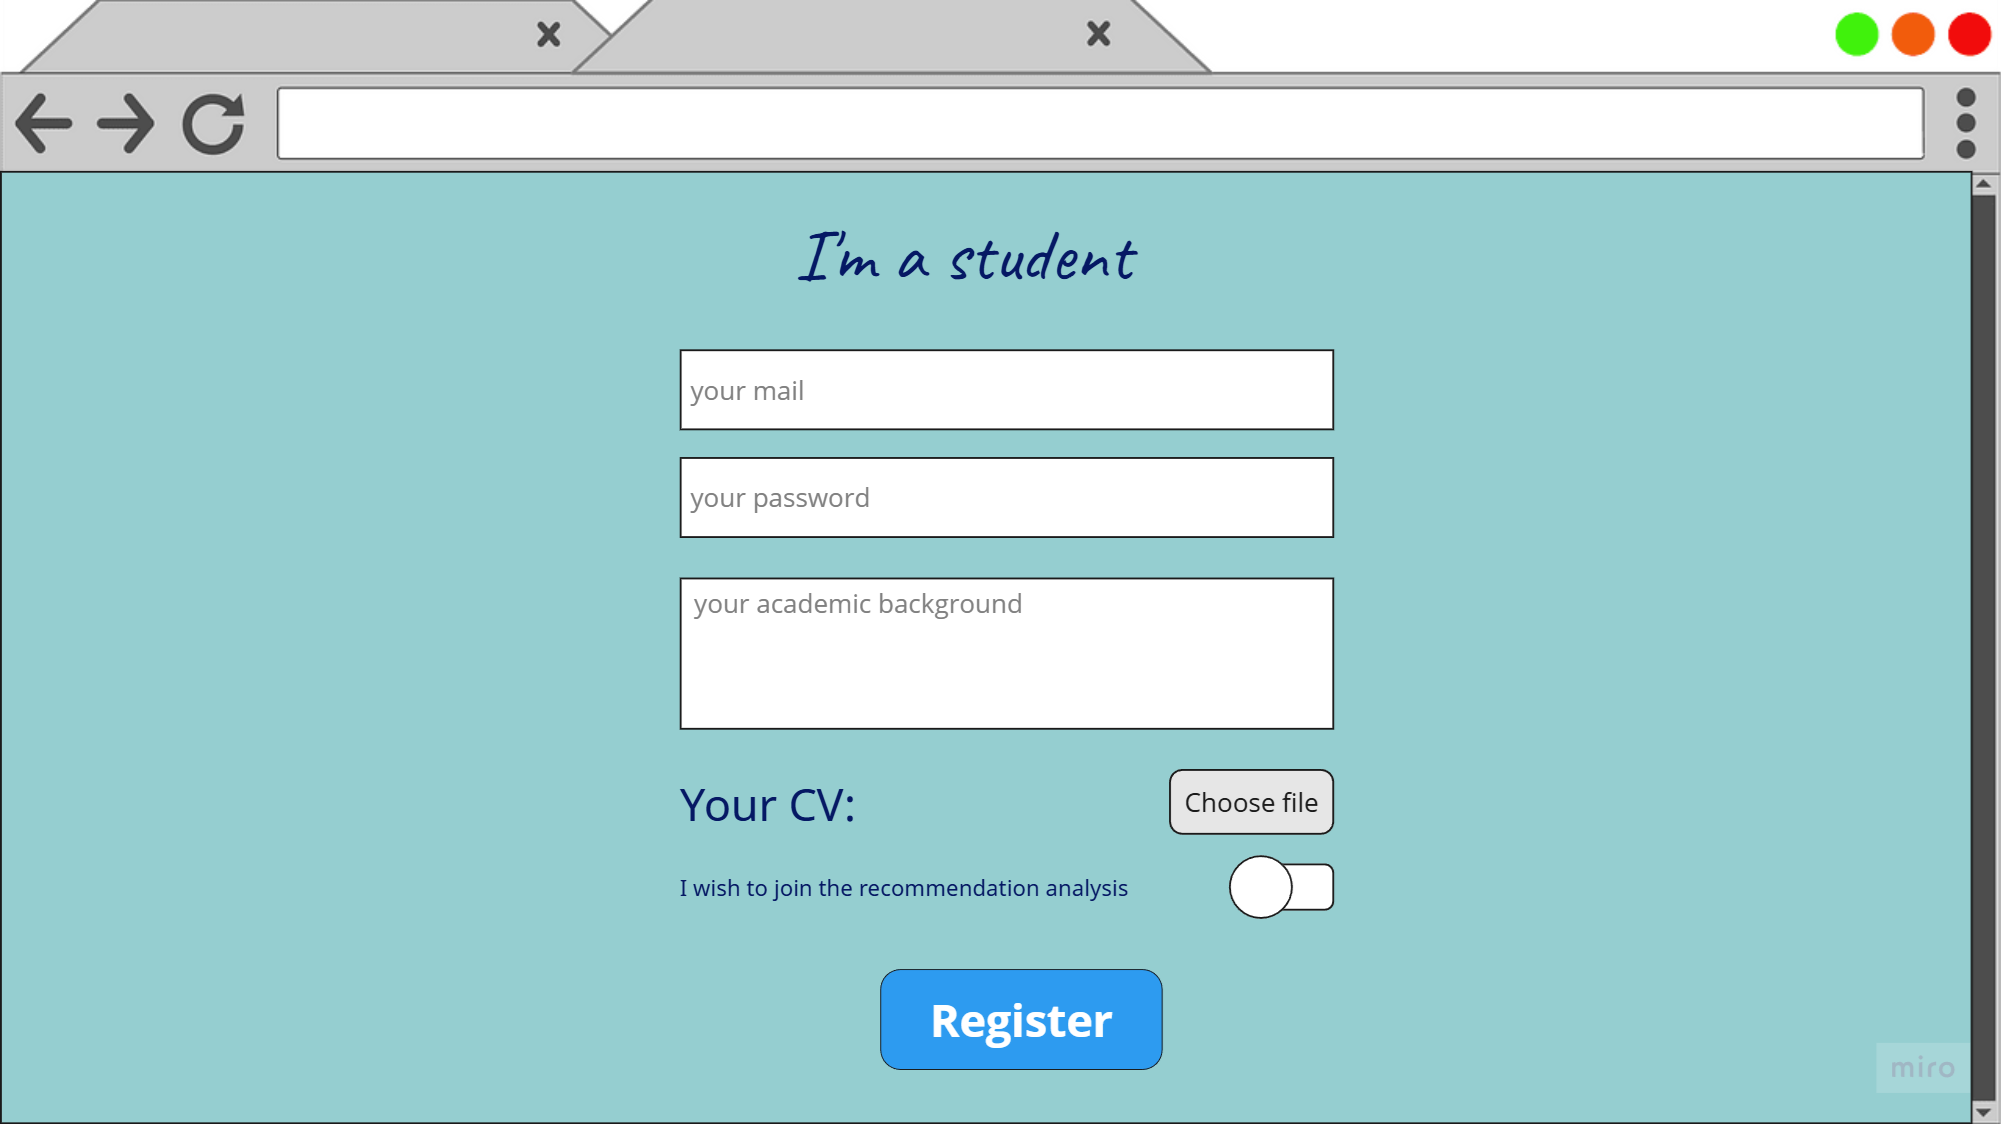
\includegraphics[width=10cm]{UI/regStudentForm.png}
	\end{figure}
	\begin{figure}[H]
		\centering
		\caption{CompanyRegistrationPage mock-up}
		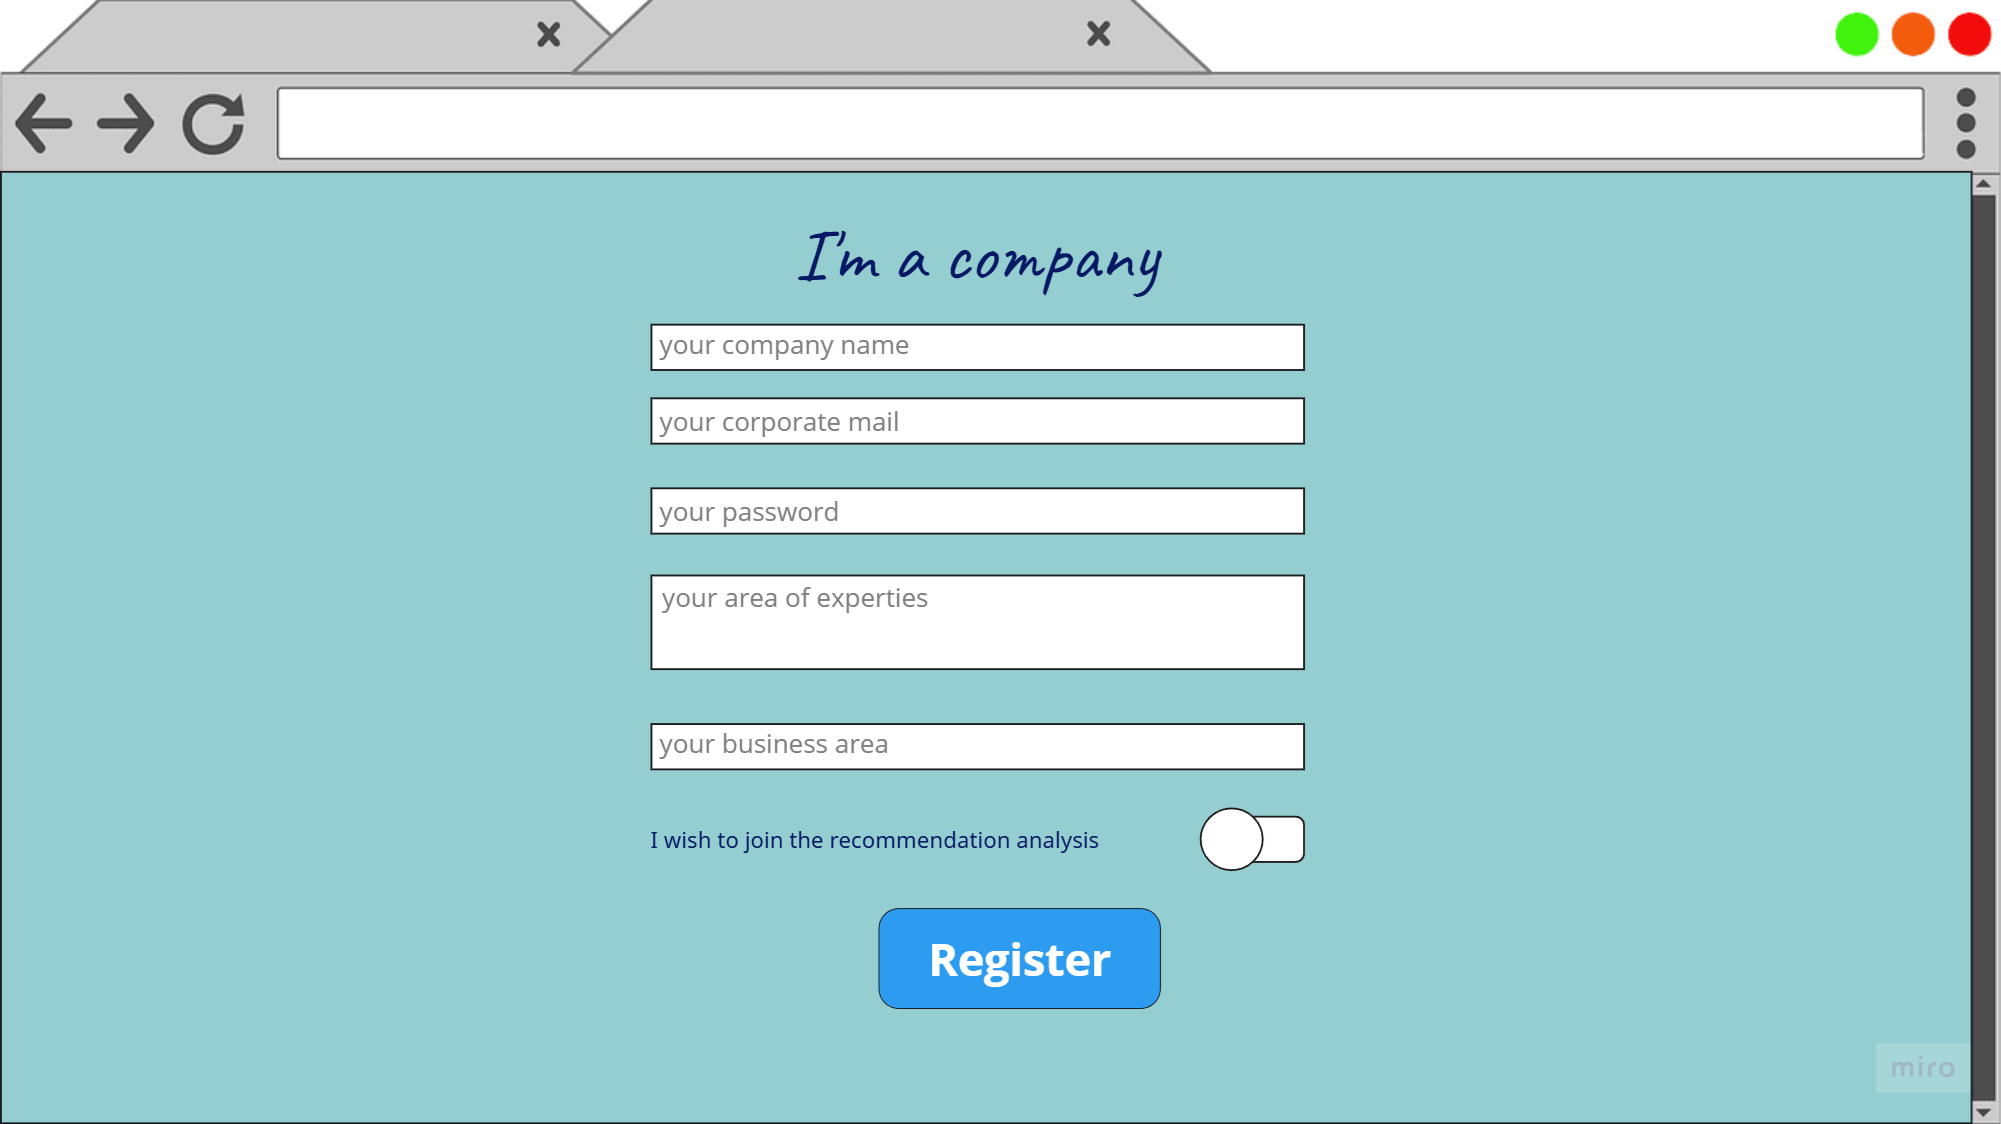
\includegraphics[width=10cm]{UI/regCompanyForm.png}
	\end{figure}
	\subsection{Login pages mock-up}
	\begin{figure}[H]
		\centering
		\caption{LoginPage mock-up}
		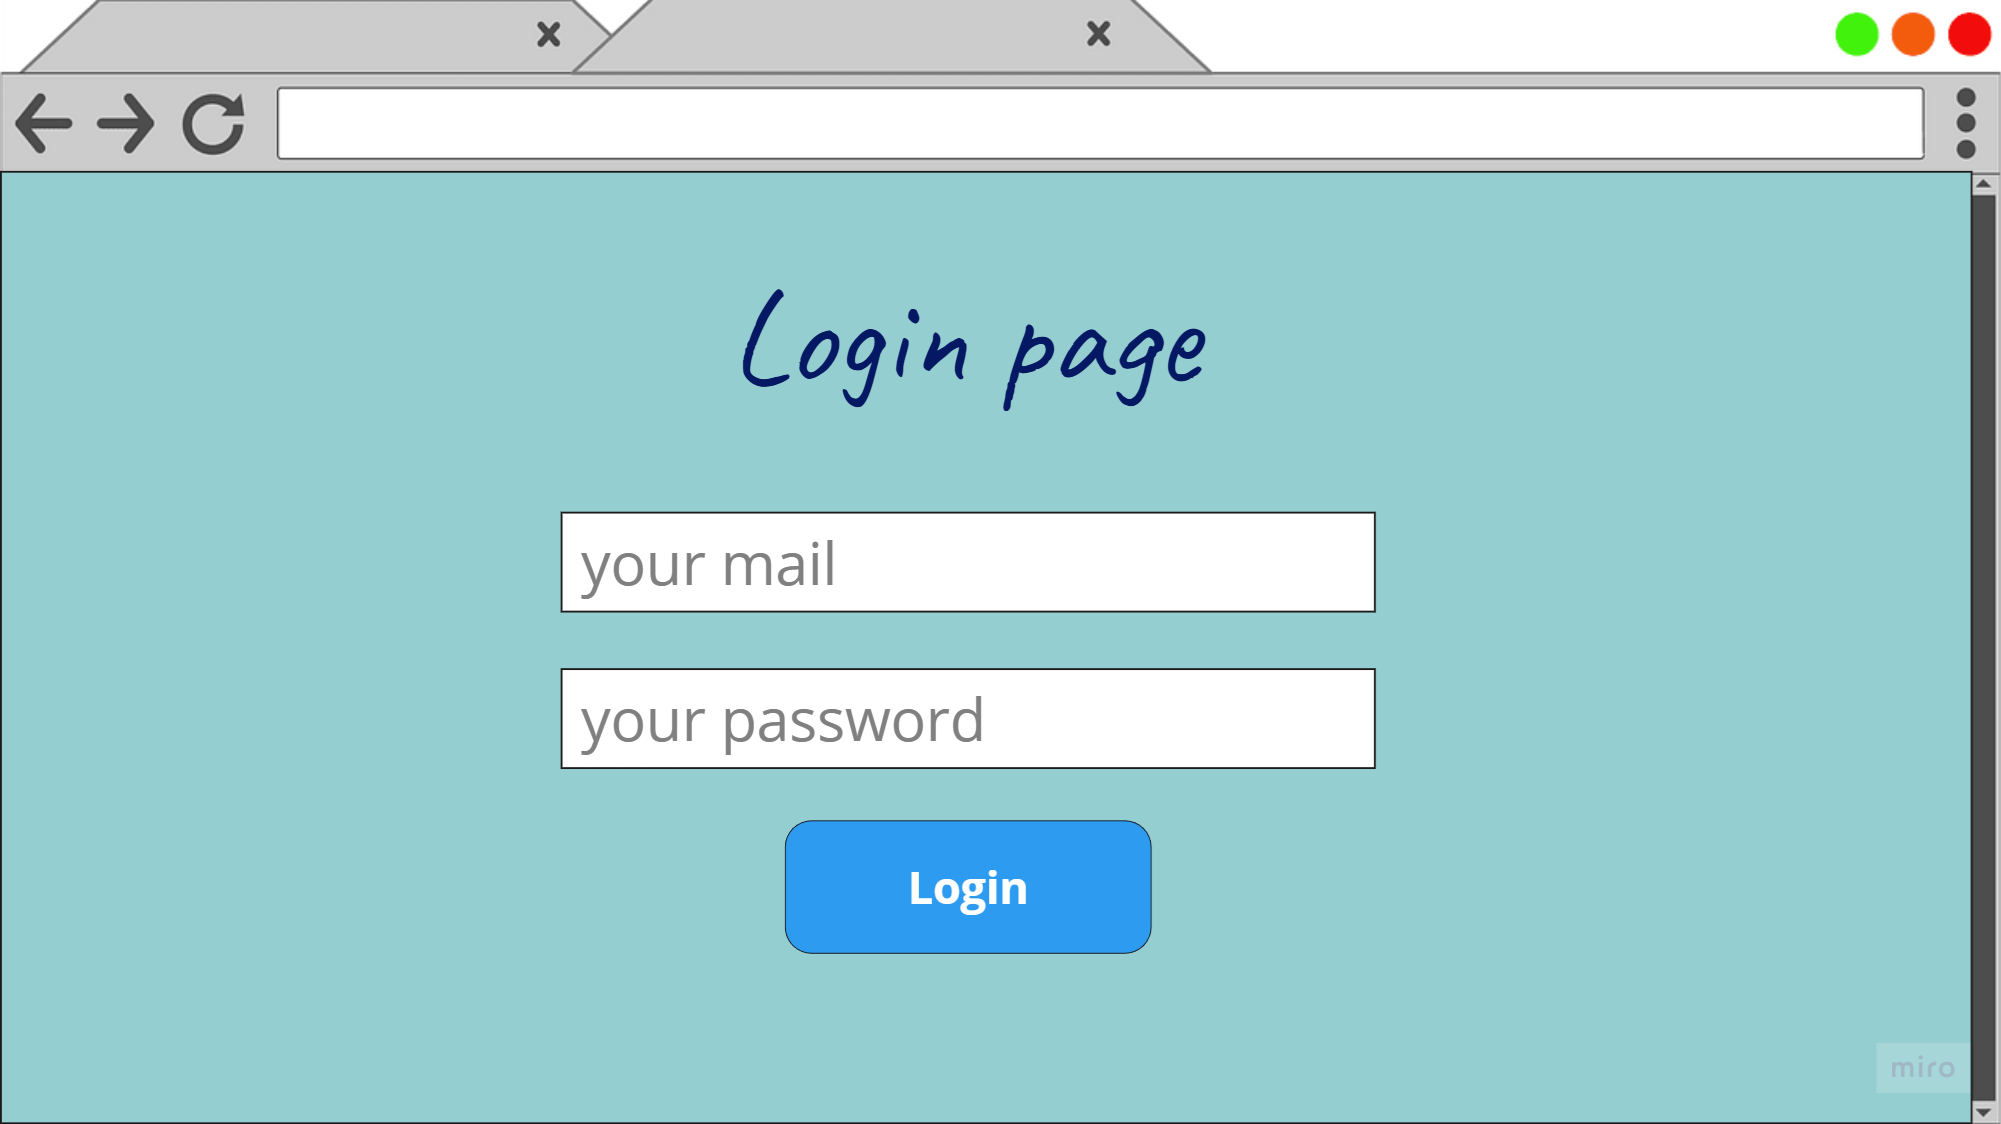
\includegraphics[width=10cm]{UI/loginPage.png}
	\end{figure}
	\section{Private pages}
	Note that for what concerns user navigation in private pages:
	\begin{itemize}
		\item as mock-up show, private sections can be accessed by means of a side-bar (this explains why navigation maps are not connected graphs);
		\item navigation maps present the designated possibilities to navigate throw sections, while mock-ups often omit navigation buttons/links (e.g. InternshipDetailsPage $\rightarrow$ CompanyProfilePage). Therefore, to implement navigation hyperlinks always refer to maps.
	\end{itemize}
	\subsection{Private pages students navigation map}
	\begin{figure}[H]
		\centering
		\caption{Private pages students navigation map}
		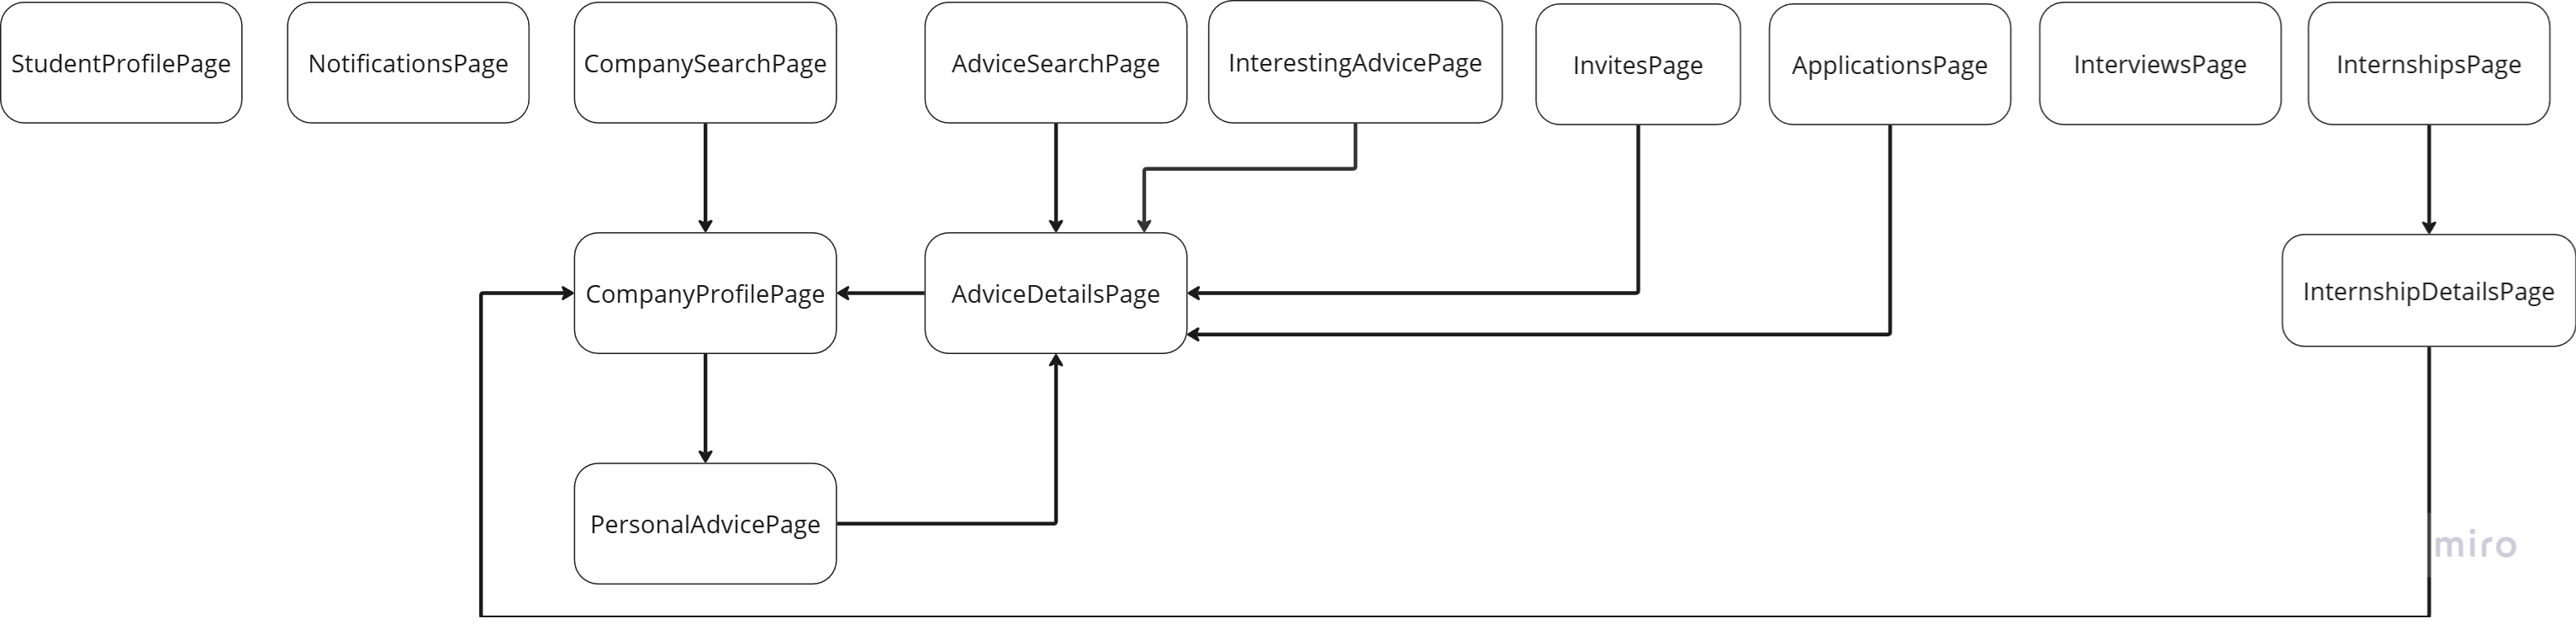
\includegraphics[width=15cm]{UI/privateStudent.png}
	\end{figure}
	\subsection{Private pages companies navigation map}
	\begin{figure}[H]
		\centering
		\caption{Private pages companies navigation map}
		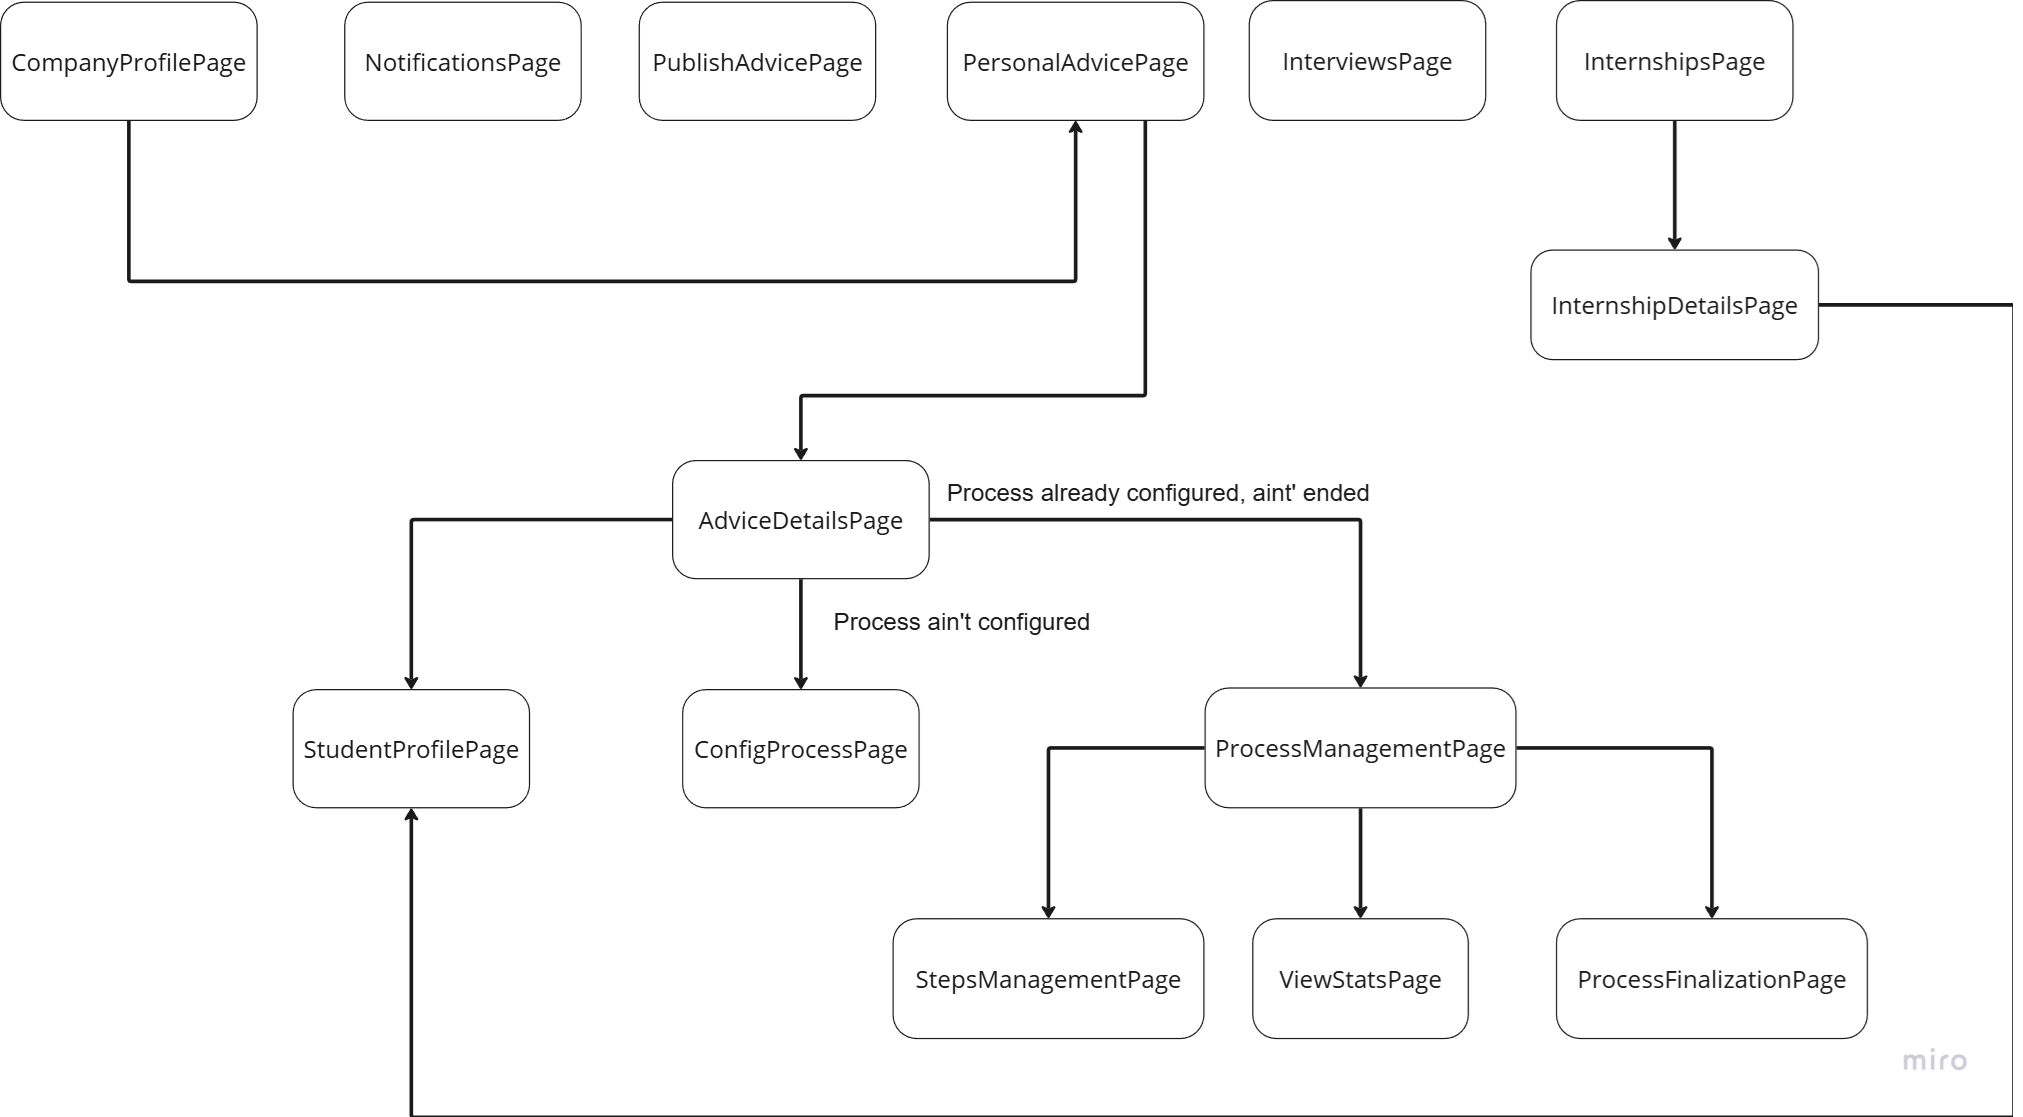
\includegraphics[width=15cm]{UI/companyPrivate.png}
	\end{figure}
	\subsection{Profile pages}
	\subsubsection{Profile pages mock-up}
	\begin{figure}[H]
		\centering
		\caption{Profiles pages (students above, companies below) mock-up from the profile's owner view point}
		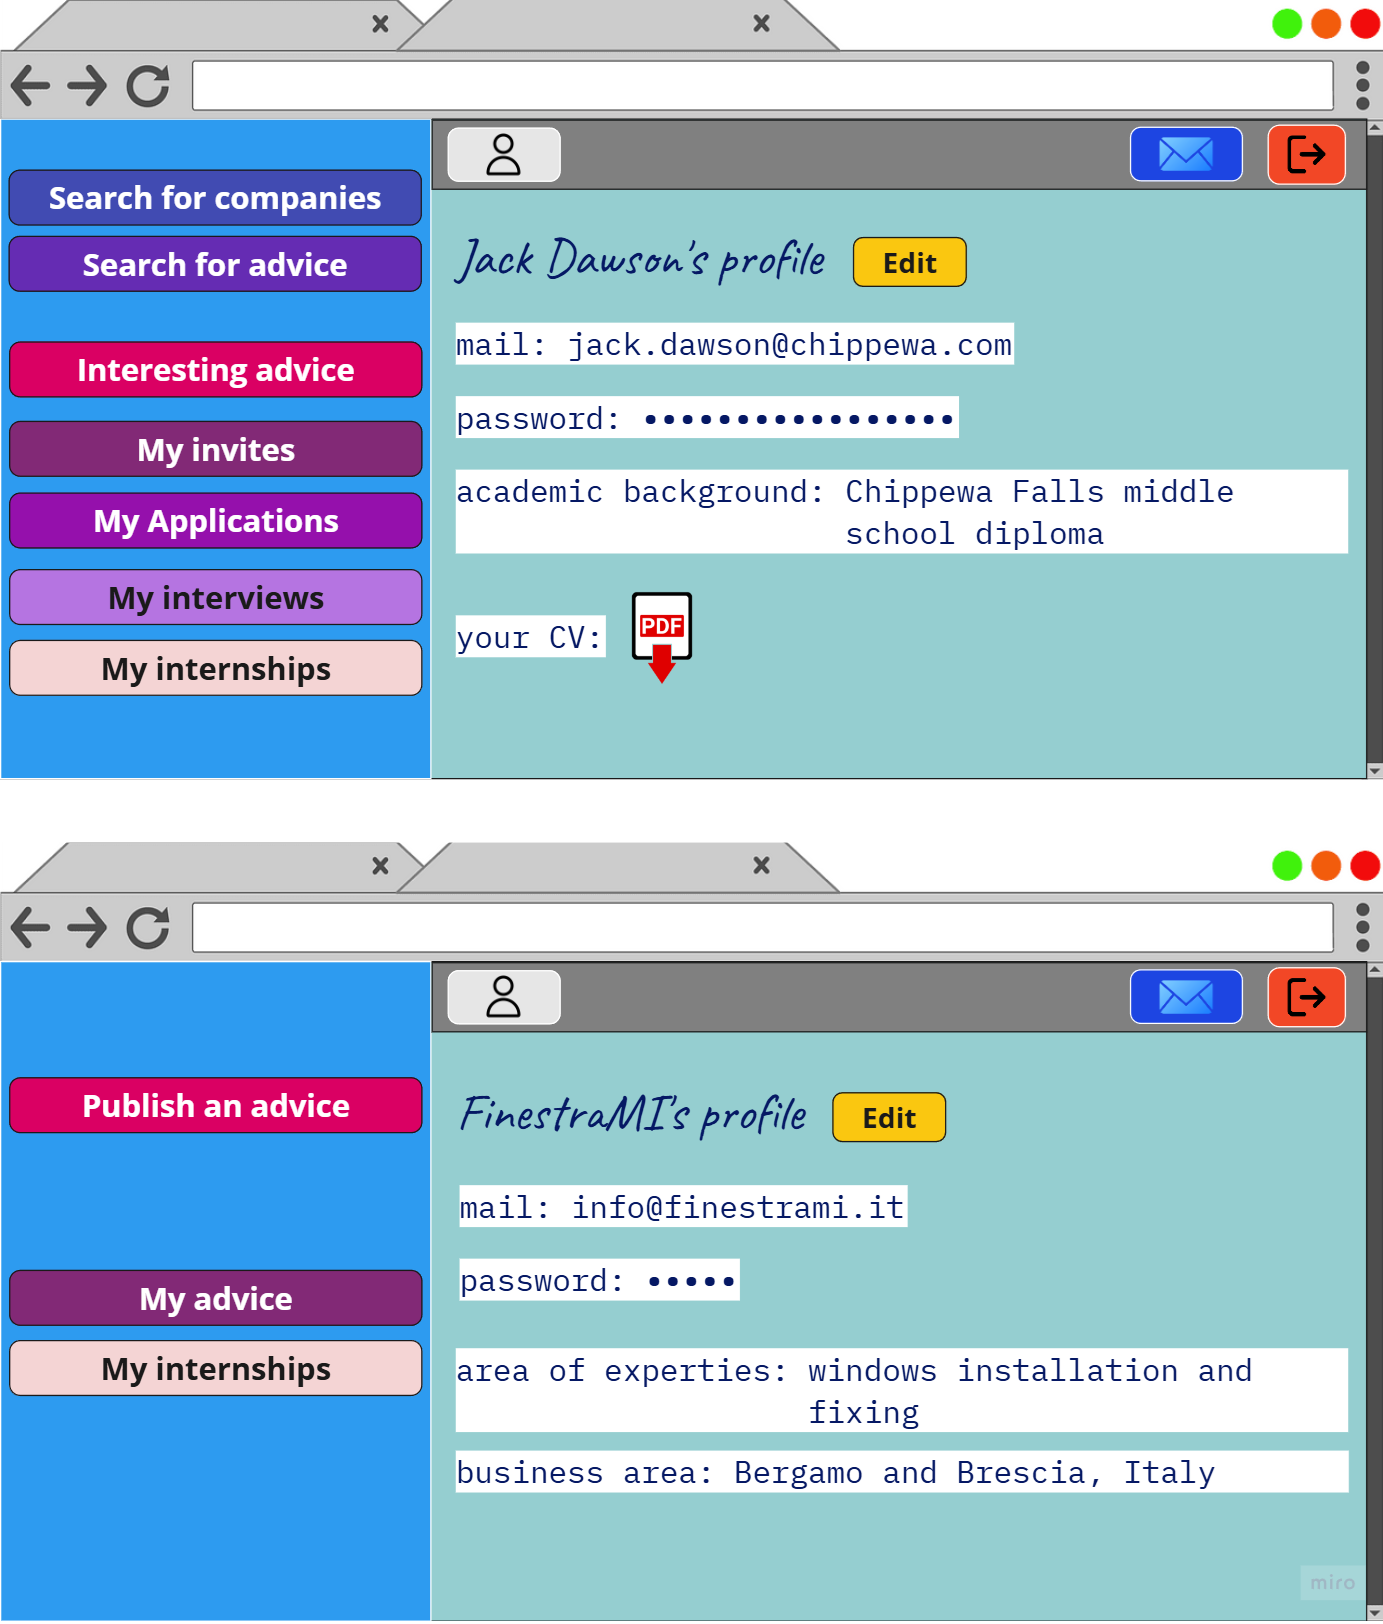
\includegraphics[width=11cm]{UI/profilesPages.png}
	\end{figure}
	\begin{figure}[H]
		\centering
		\caption{Profiles pages (students on the left, companies on the right) mock-up from other users view point}
		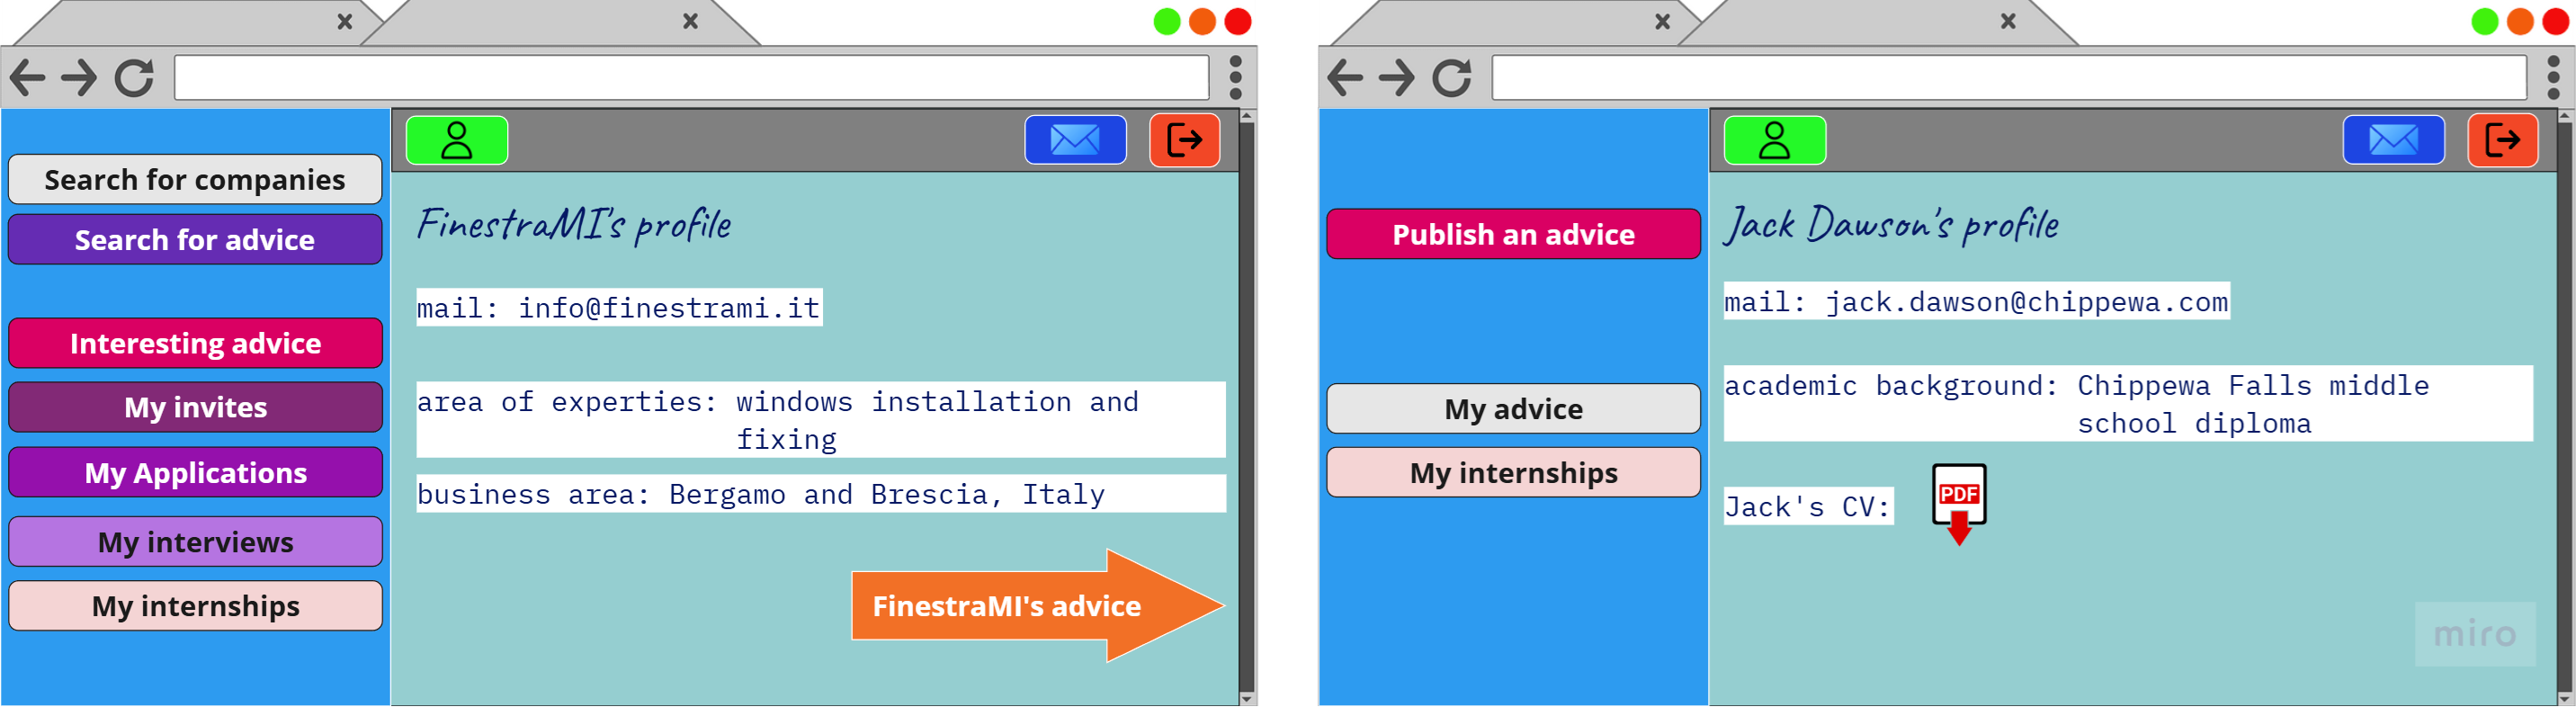
\includegraphics{UI/profilesPagesPublic.png}
	\end{figure}
	\subsection{Notifications pages}
	\subsubsection{Notifications pages mock-up}
	\begin{figure}[H]
		\centering
		\caption{NotificationsPage and Notification modal box mock-up}
		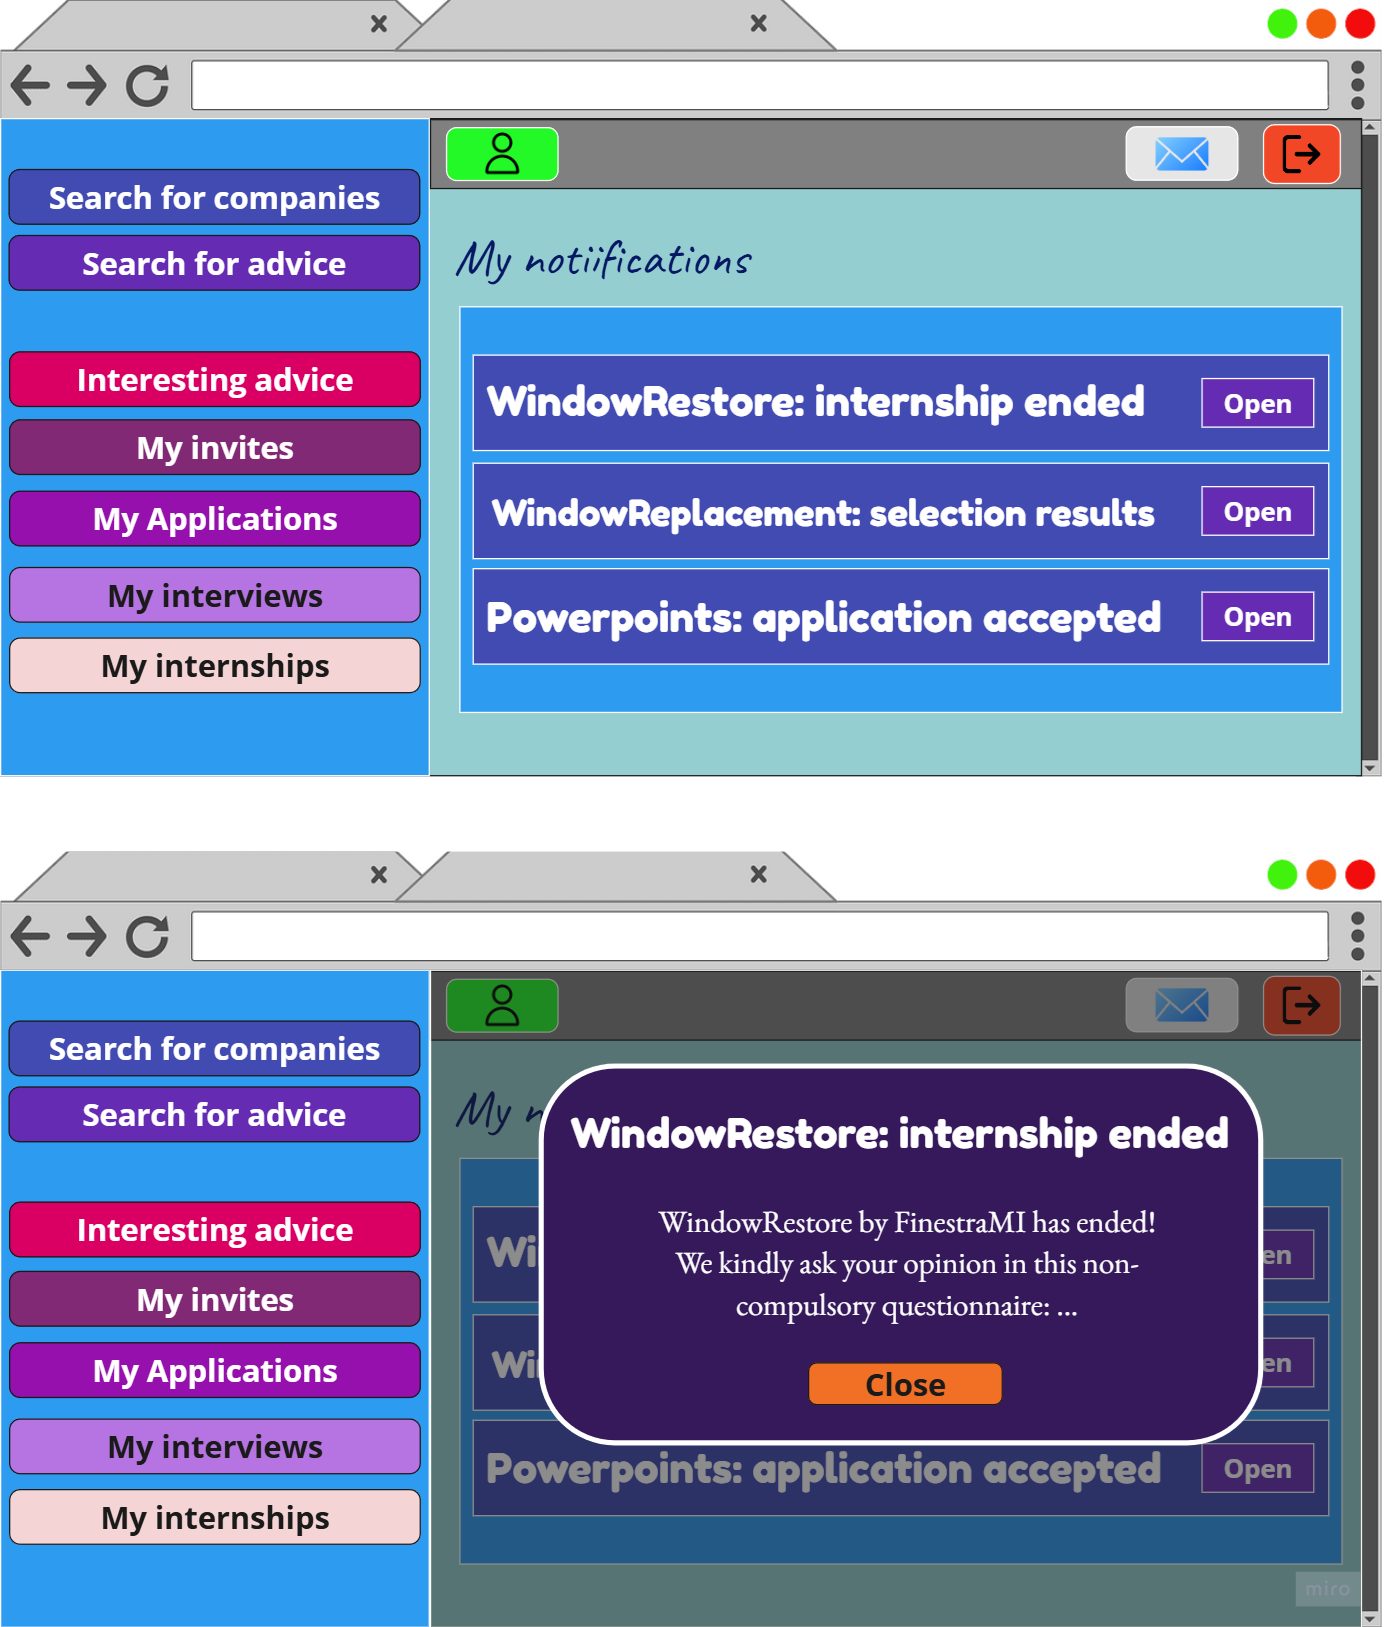
\includegraphics[width=11cm]{UI/notifications.png}
	\end{figure}
	Non-compulsory questionnaires are shown on a single window accessible from a link in the notification related to them:
	\begin{figure}[H]
		\centering
		\caption{Feedback questionnaire window mock-up}
		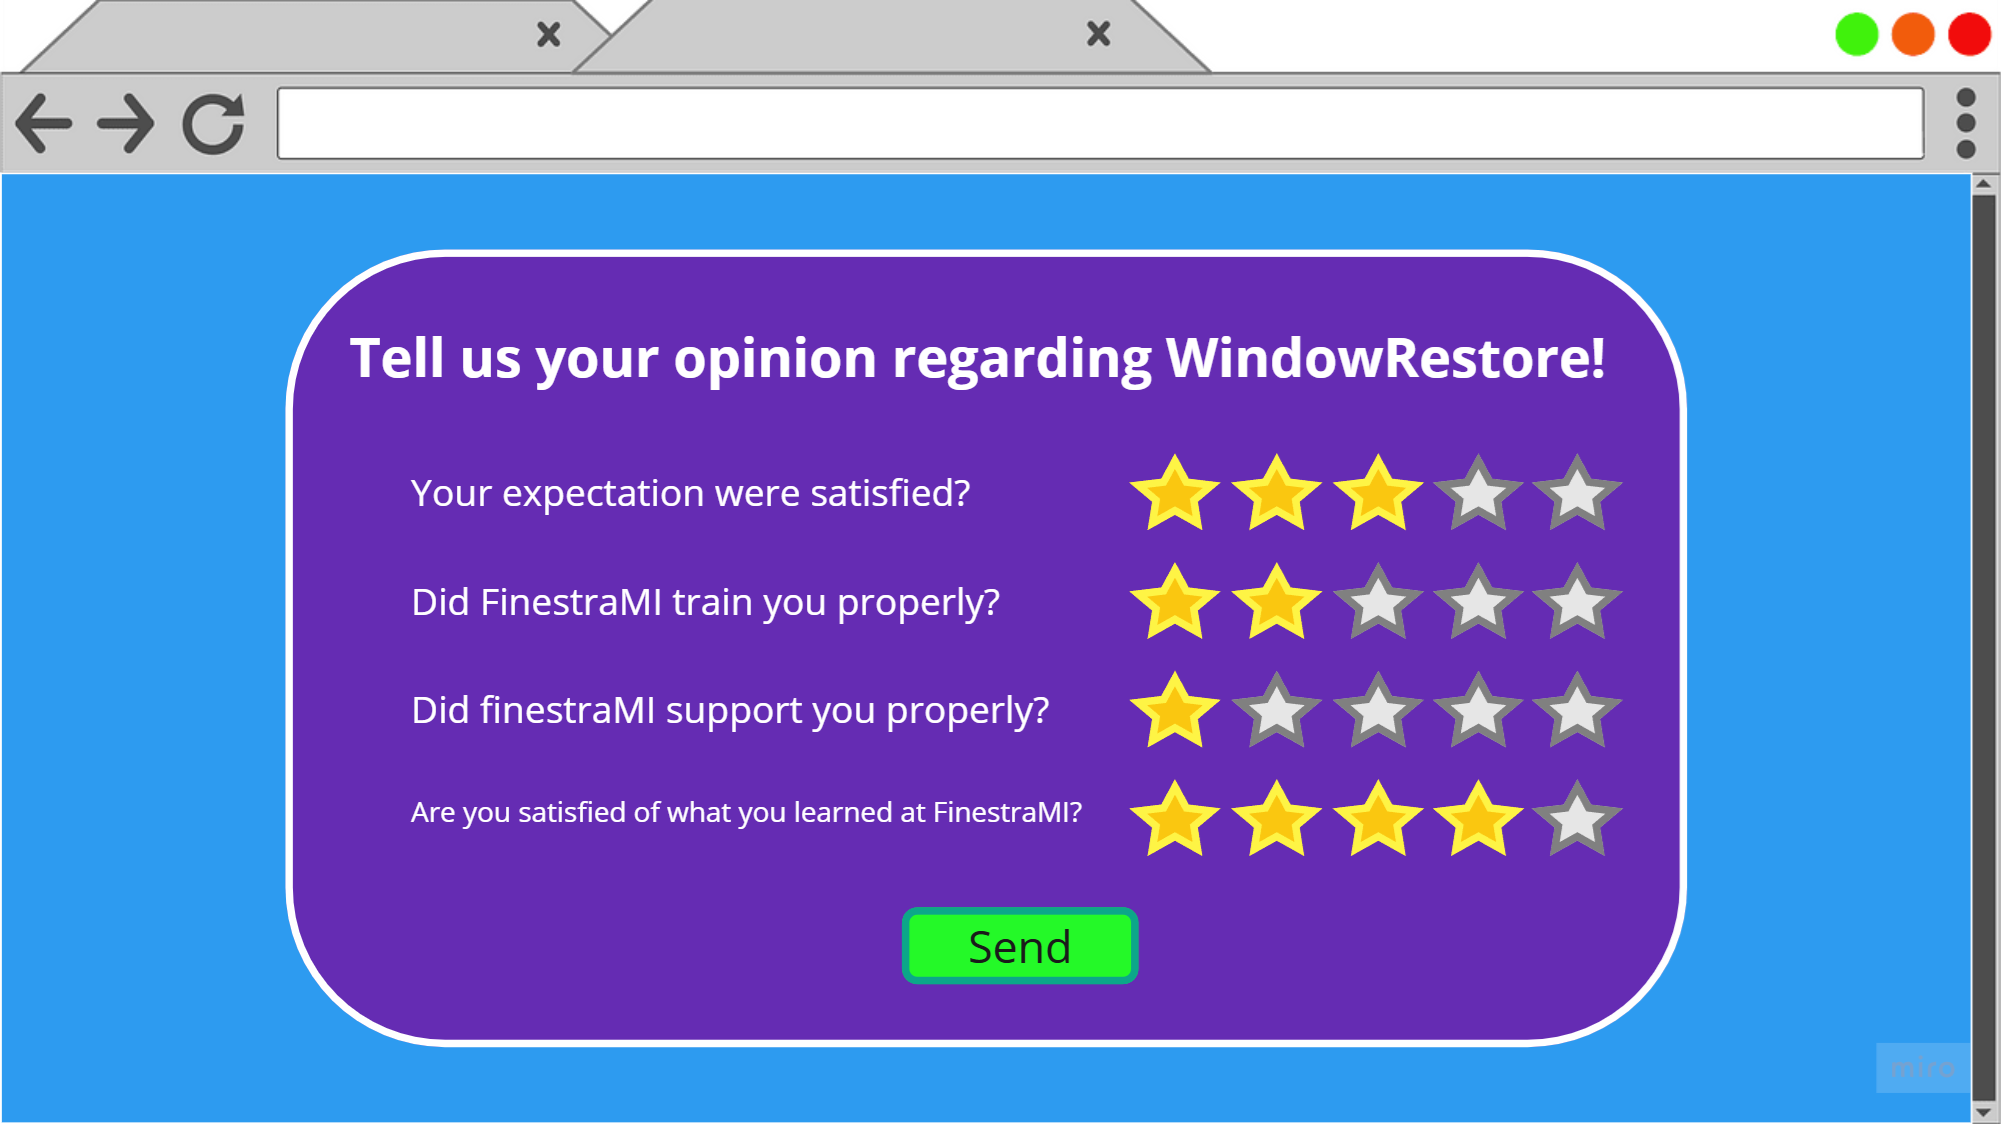
\includegraphics[width=11cm]{UI/questionnaire.png}
	\end{figure}
	\subsection{Companies pages}
	\subsubsection{Companies pages mock-up}
	\begin{figure}[H]
		\centering
		\caption{CompanySearchPage mock-up}
		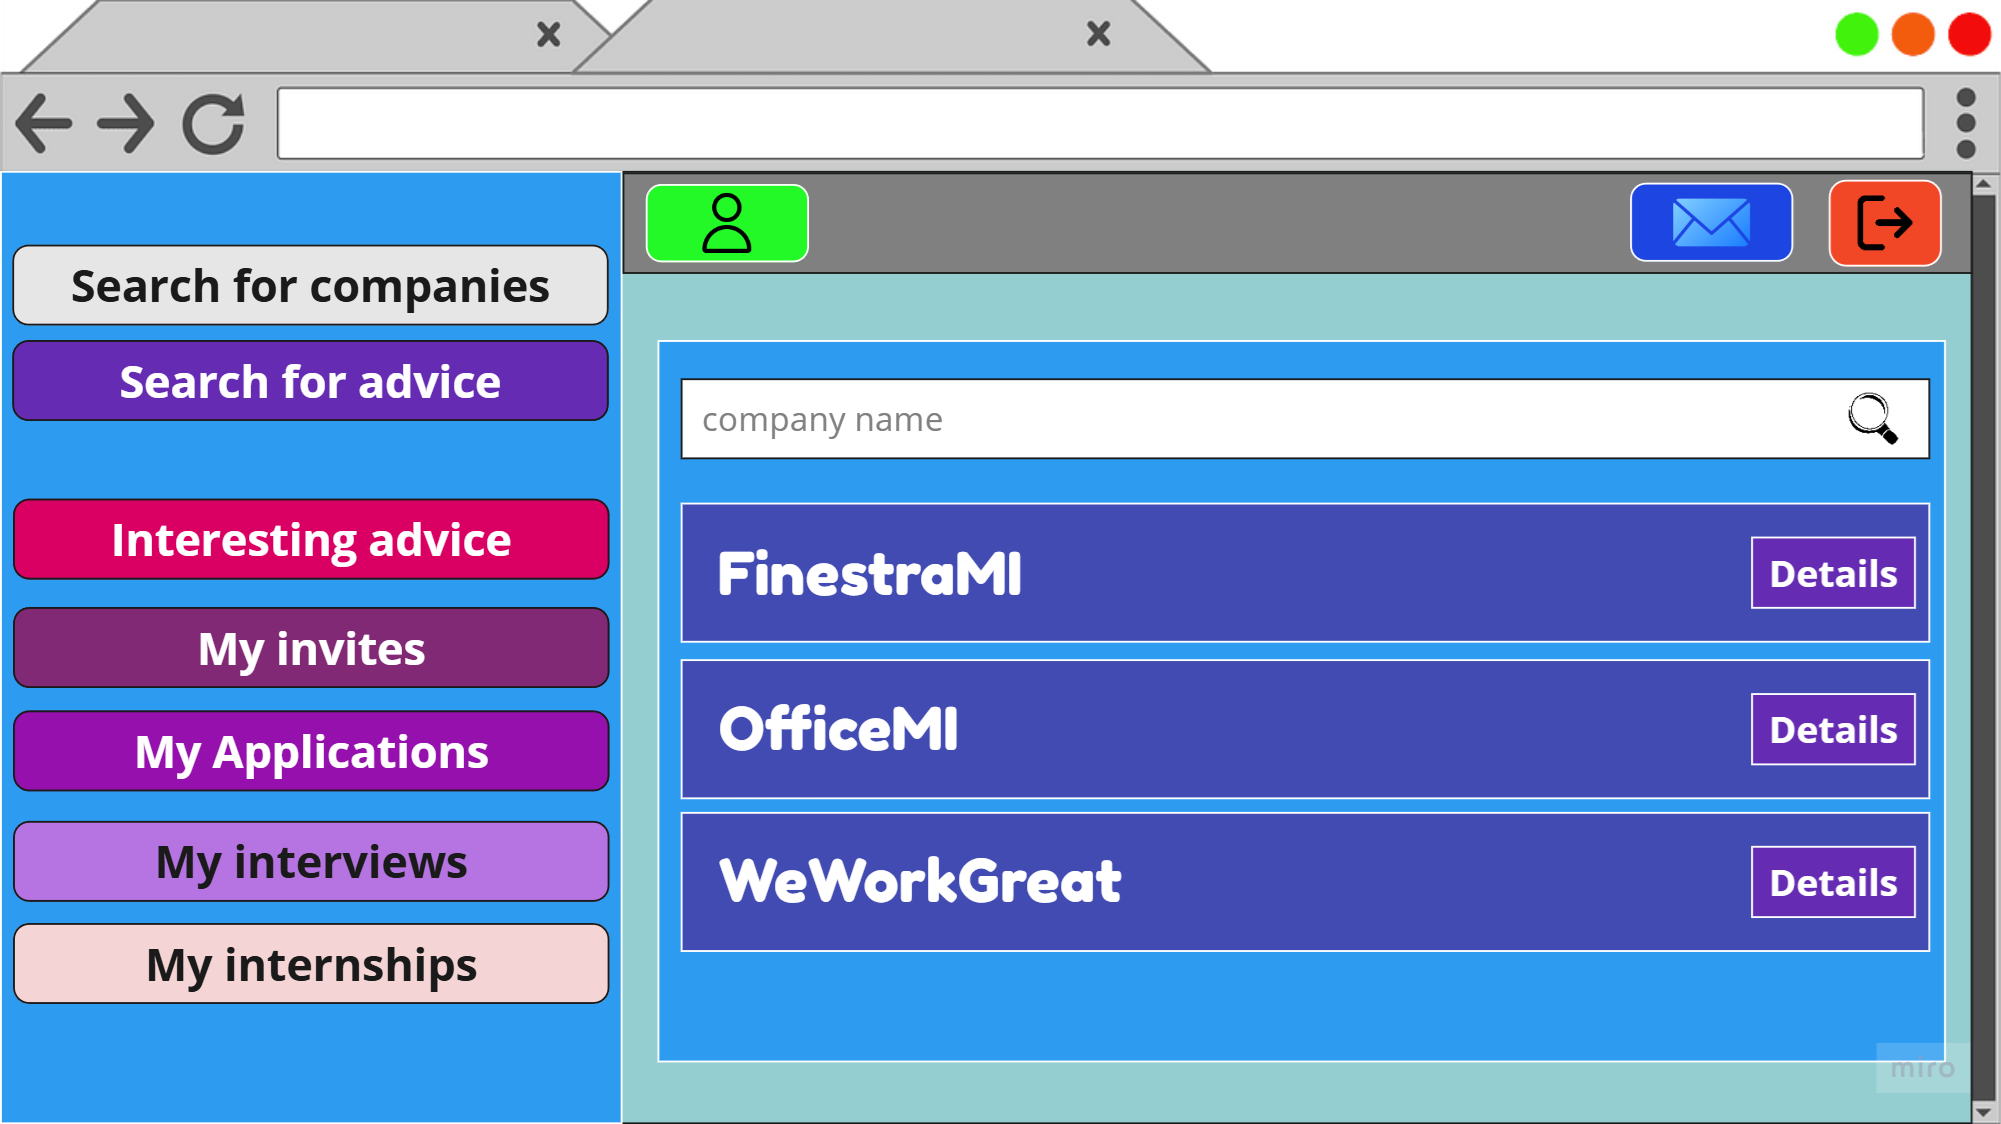
\includegraphics[width=10cm]{UI/companiesPage.png}
	\end{figure}
	\subsection{Advice-related pages}
	\subsubsection{Advice-related pages mock-up}
	\begin{figure}[H]
		\centering
		\caption{AdviceSearchPage mock-up}
		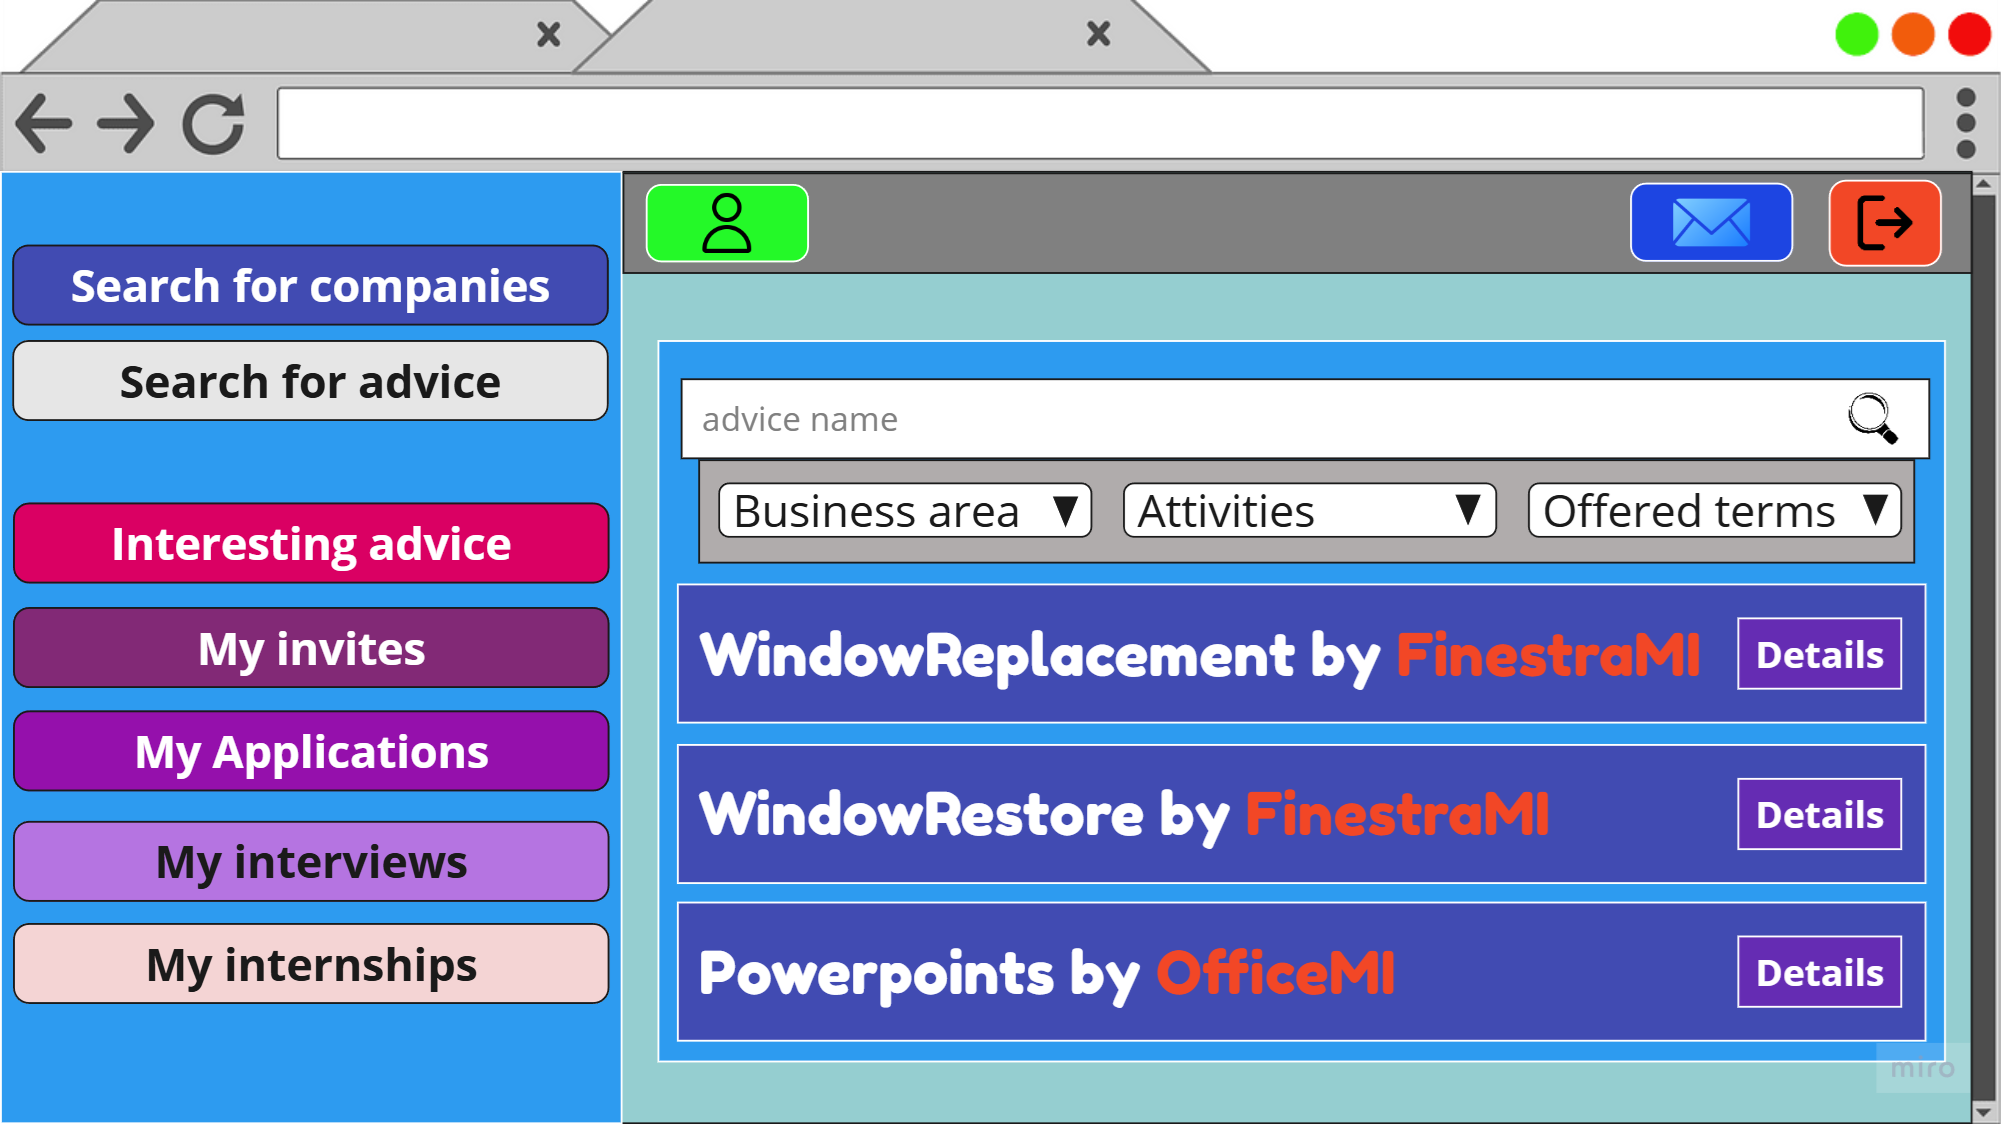
\includegraphics[width=11cm]{UI/adviceSearchPage.png}
	\end{figure}
	\begin{figure}[H]
		\centering
		\caption{PersonalAdvicePage mock-up}
		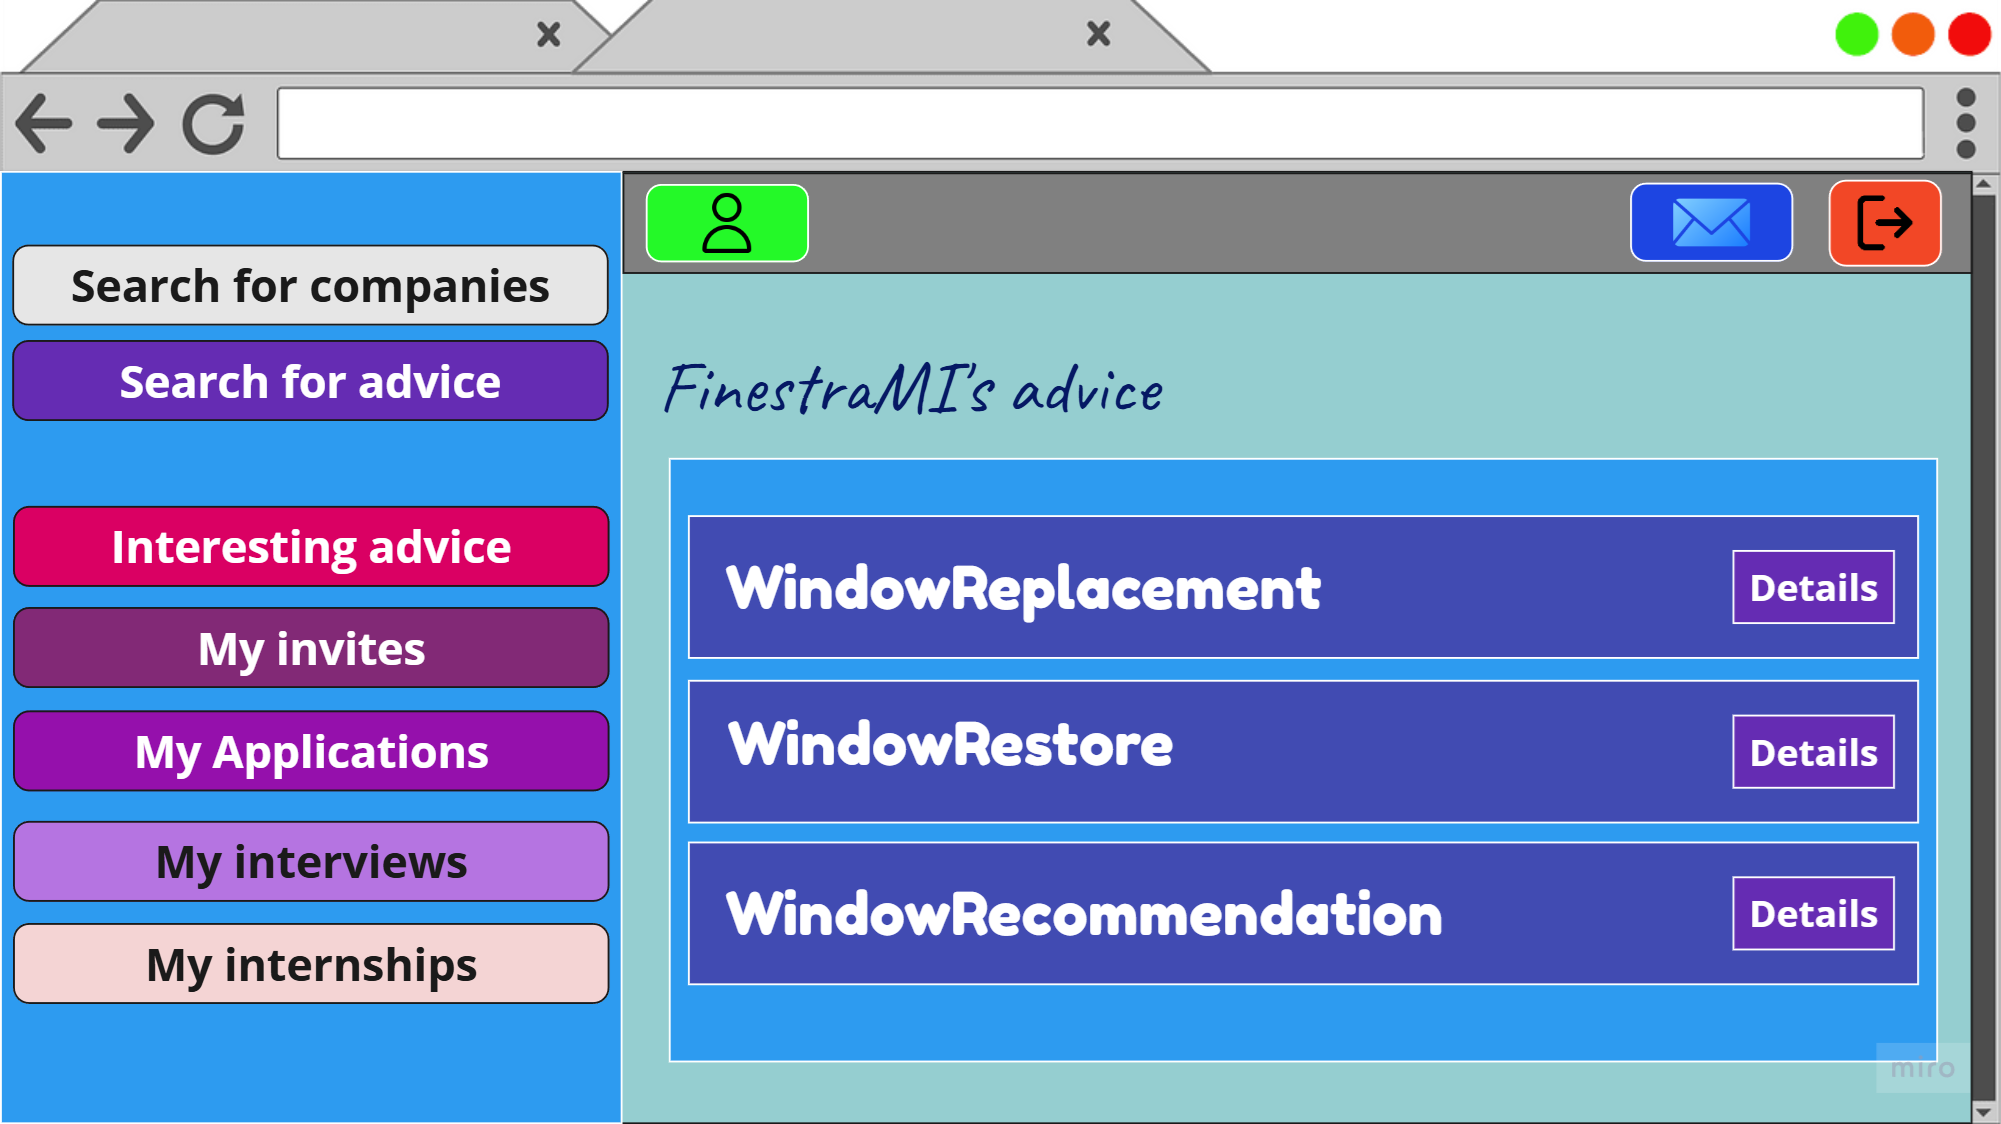
\includegraphics[width=11cm]{UI/adviceCompanyList.png}
	\end{figure}
	\begin{figure}[H]
		\centering
		\caption{PublishAdvicePage mock-up}
		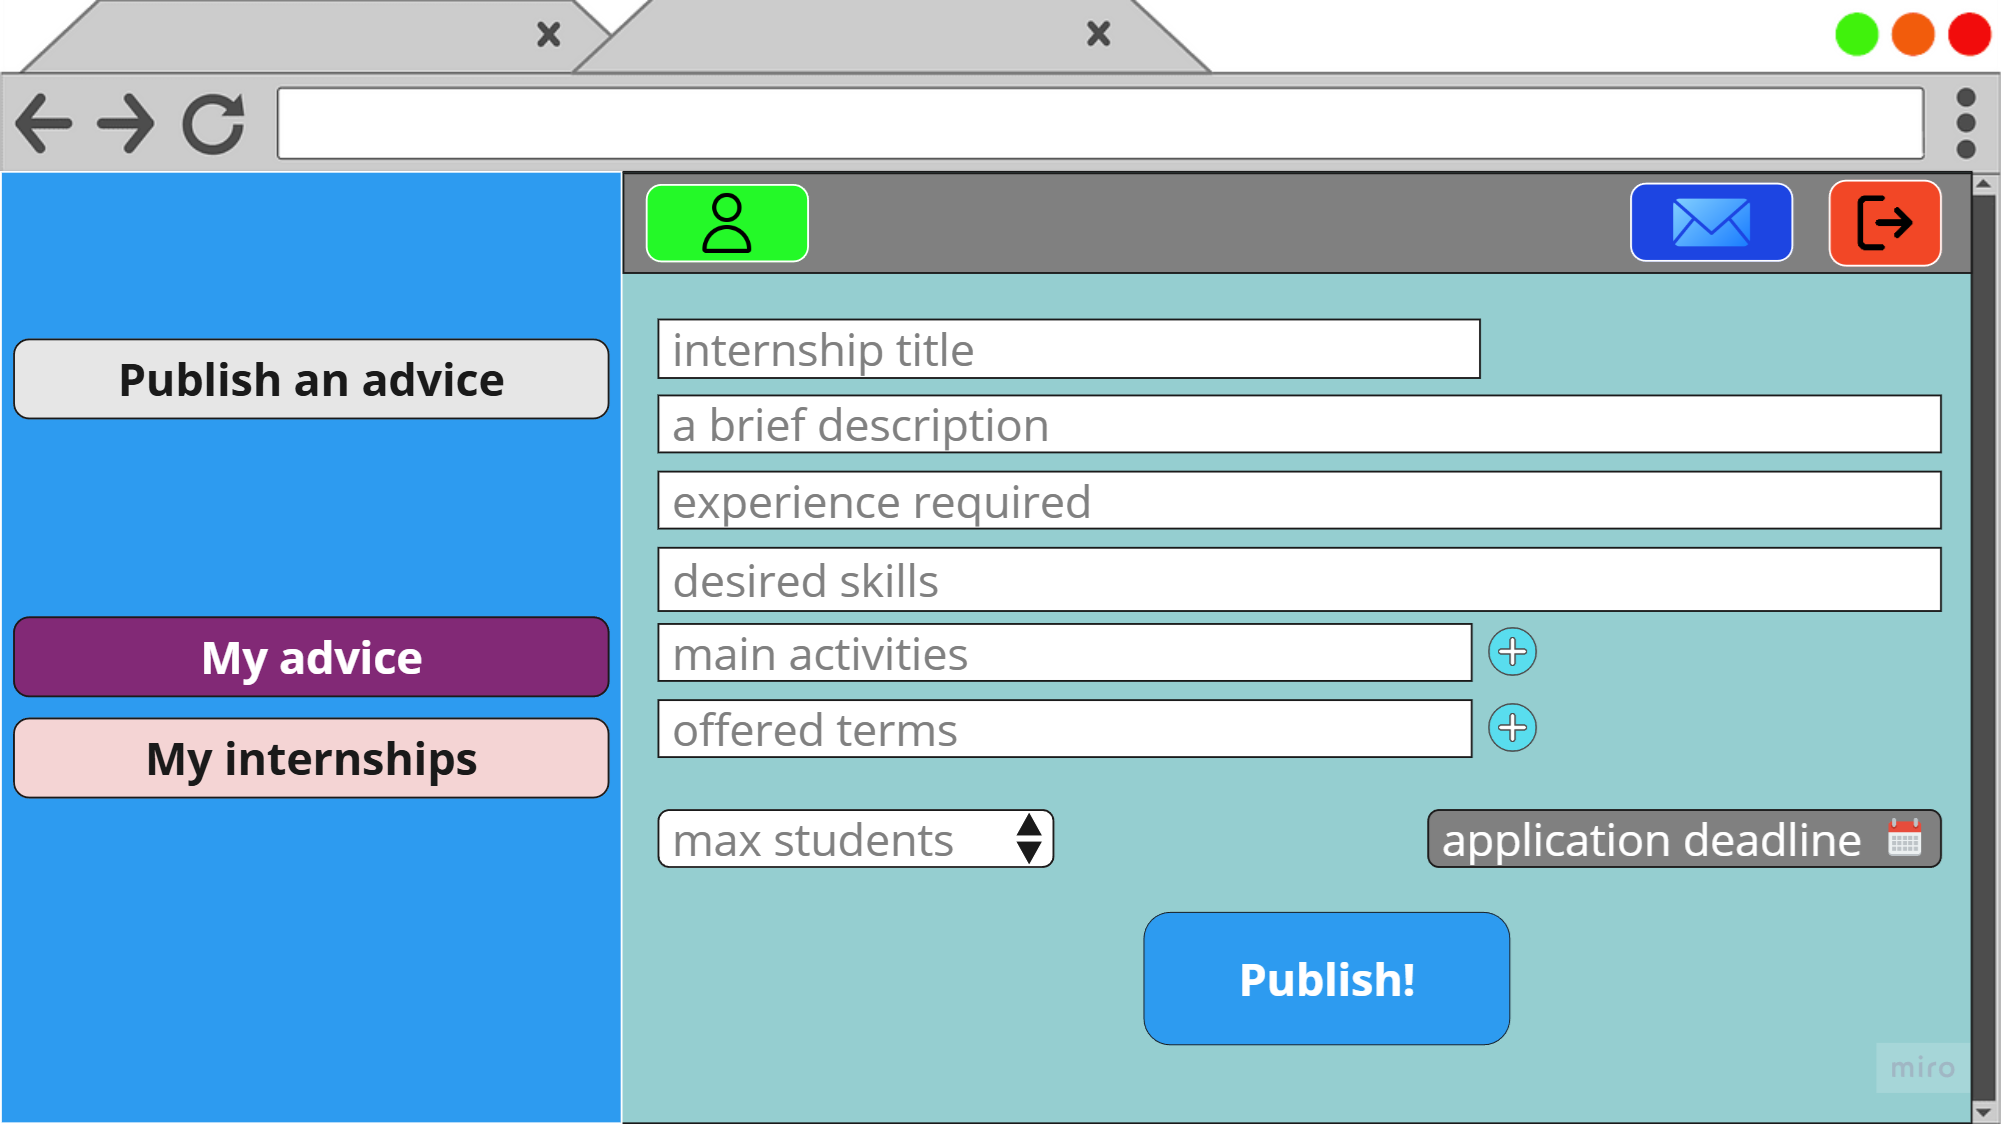
\includegraphics[width=11cm]{UI/publishAdvice.png}
	\end{figure}
	\begin{figure}[H]
		\centering
		\caption{AdviceDetailsPage (students view-point) mock-up}
		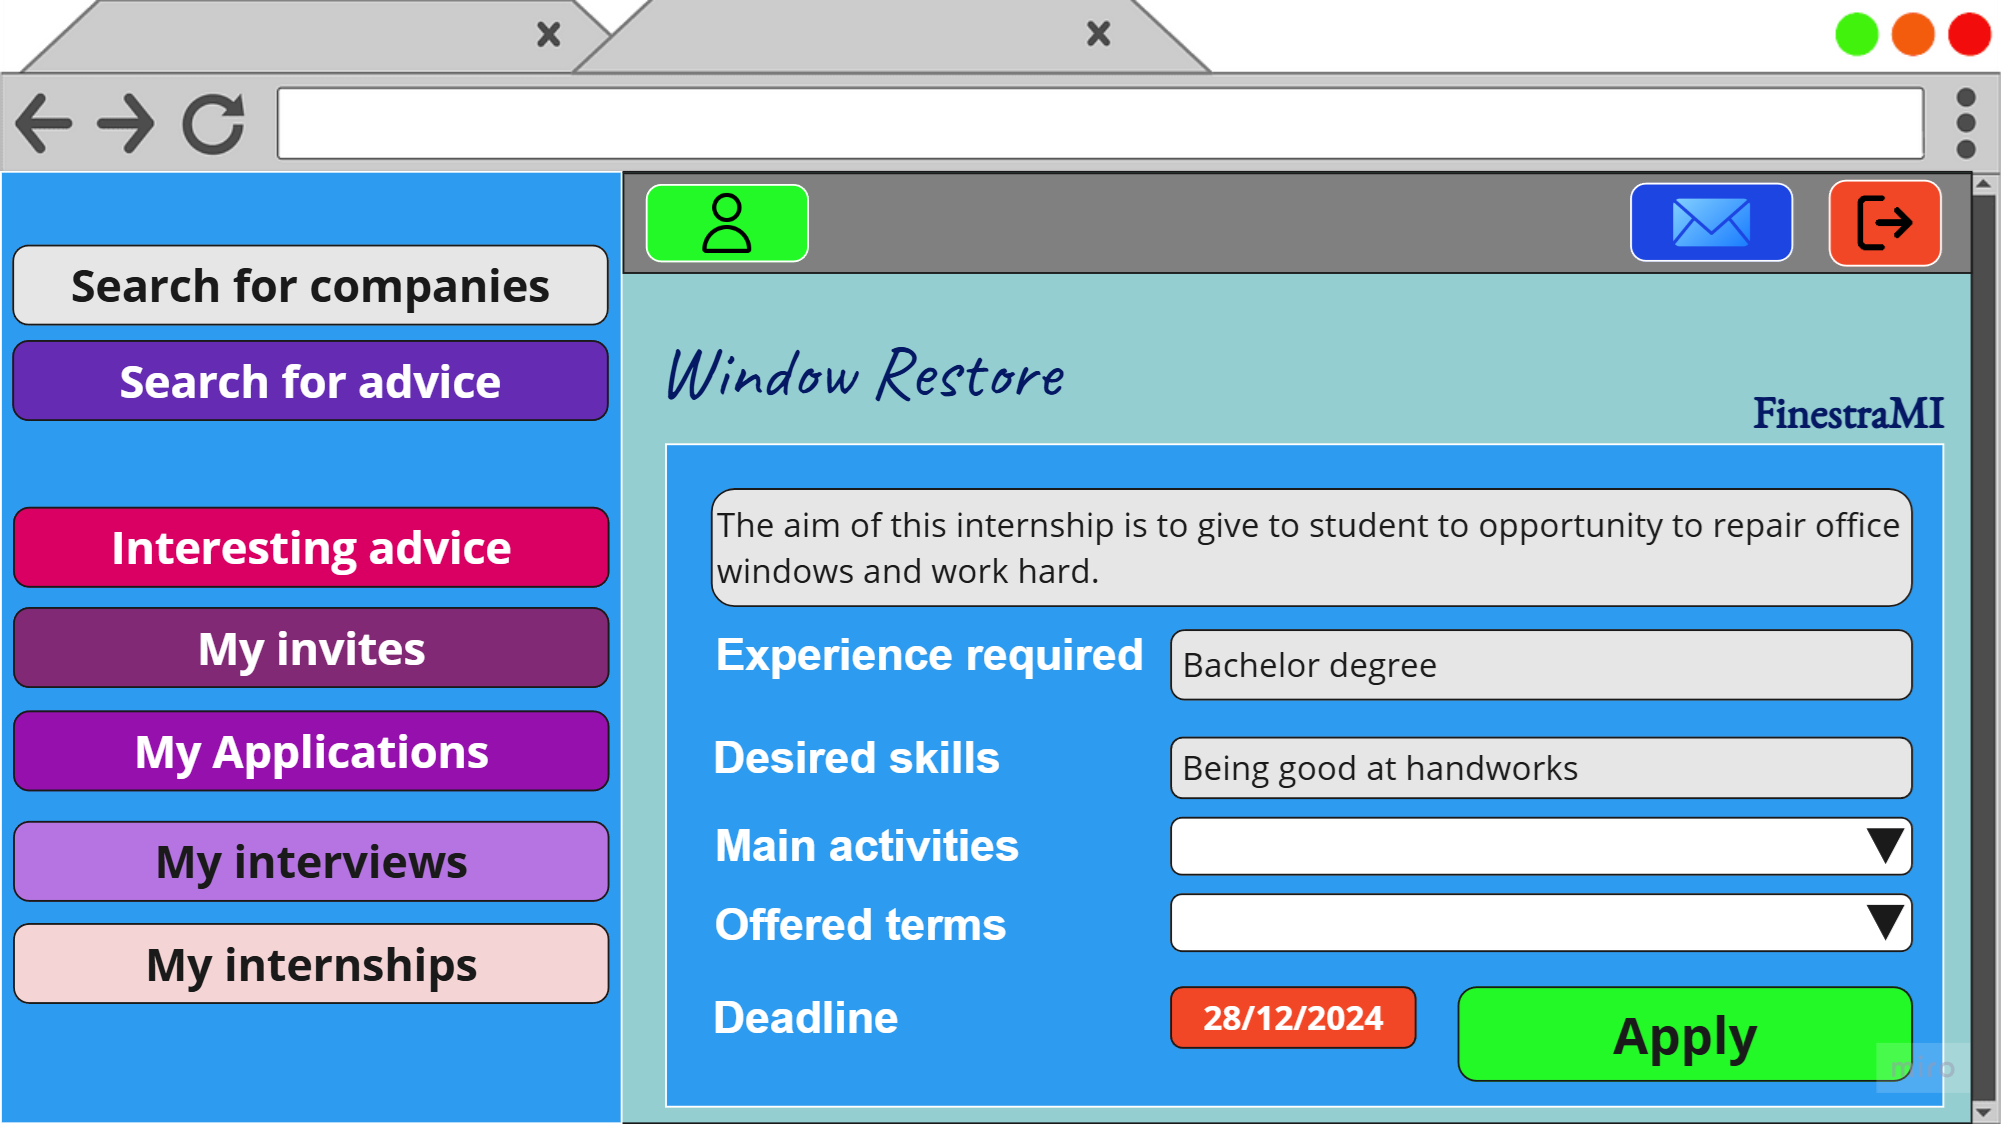
\includegraphics[width=11cm]{UI/advicePage.png}
	\end{figure}
	\begin{figure}[H]
		\centering
		\caption{AdviceDetailsPage (company view-point) mock-up}
		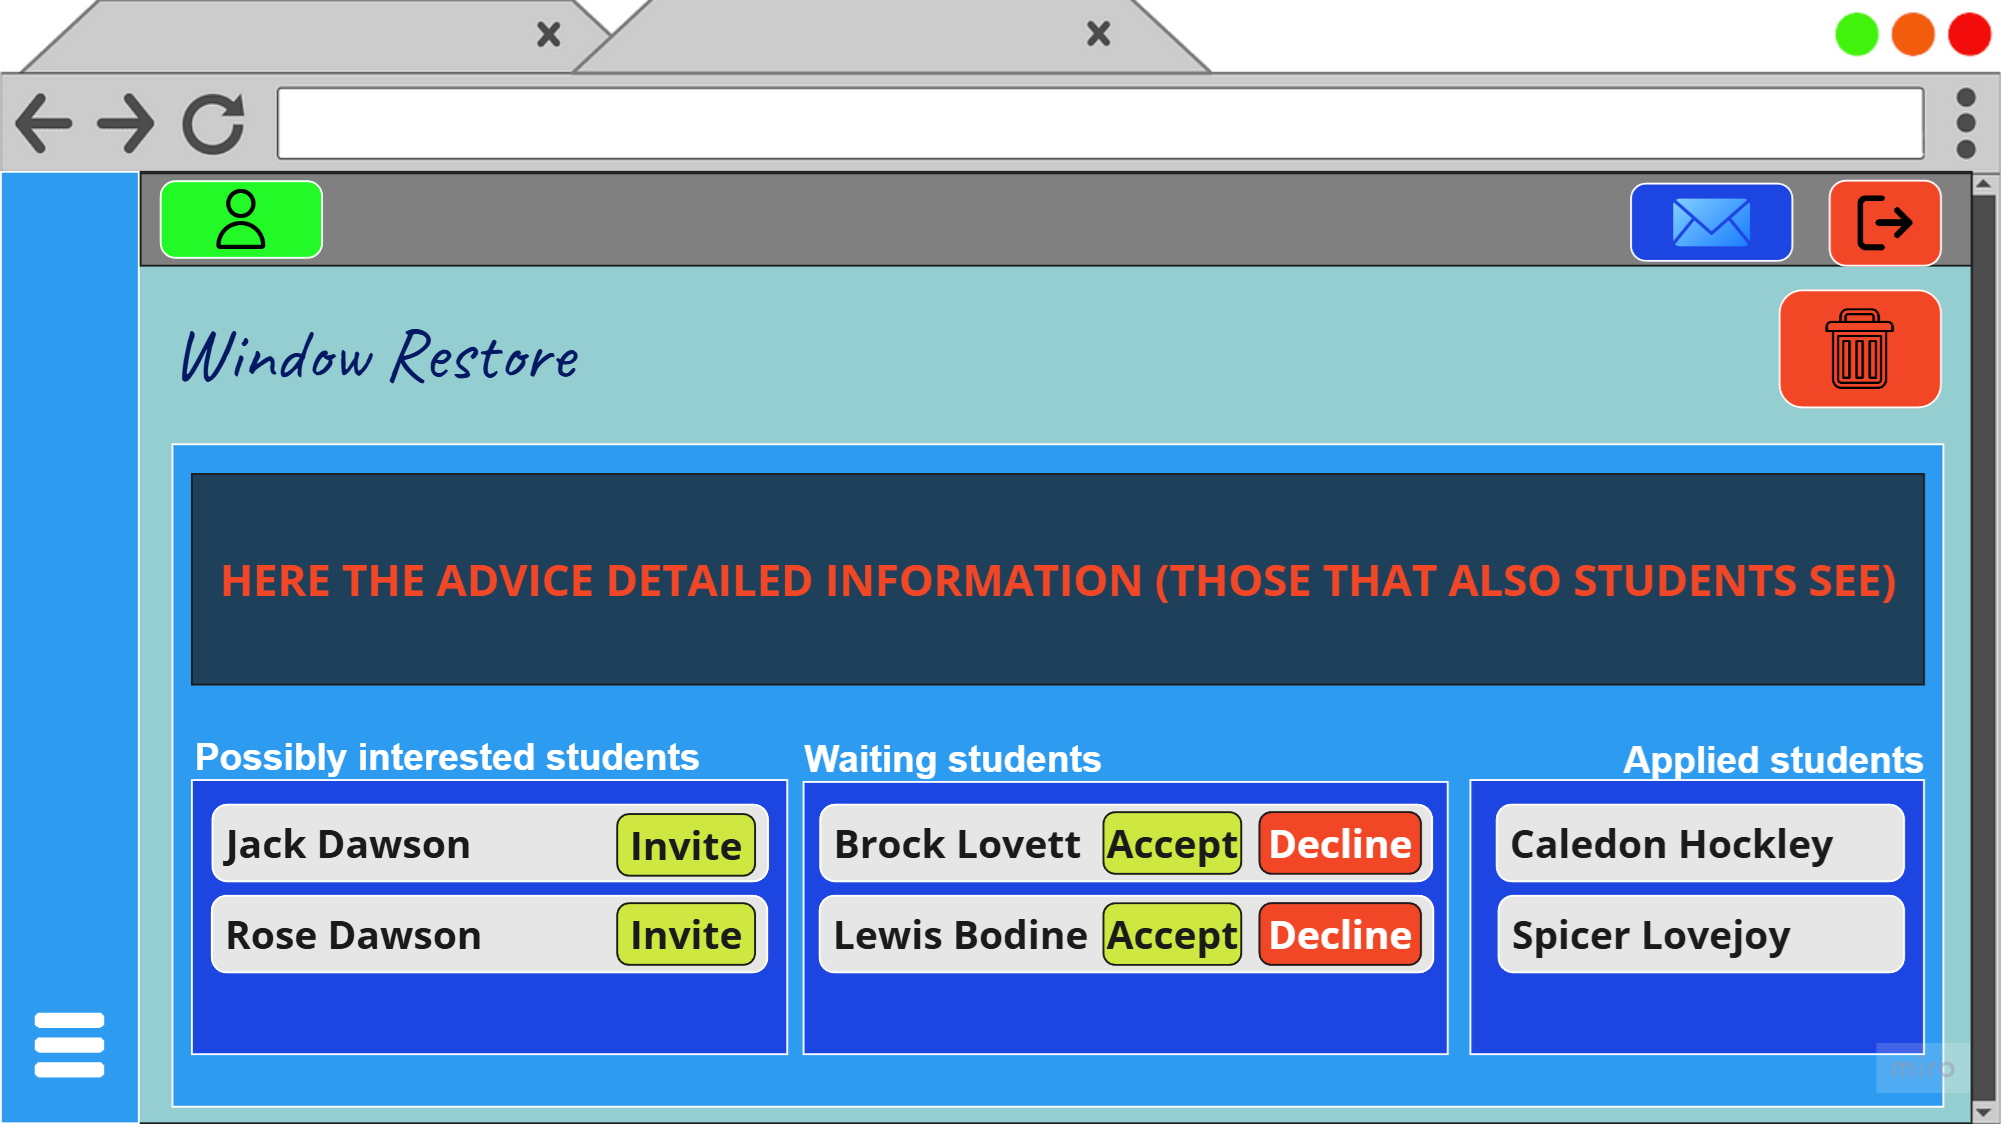
\includegraphics[width=11cm]{UI/advicePageCompany.png}
	\end{figure}
	The trash button will turn into a \emph{Configure selection process} button once the advice deadline has last.
	\begin{figure}[H]
		\centering
		\caption{InterestingAdvicePage mock-up}
		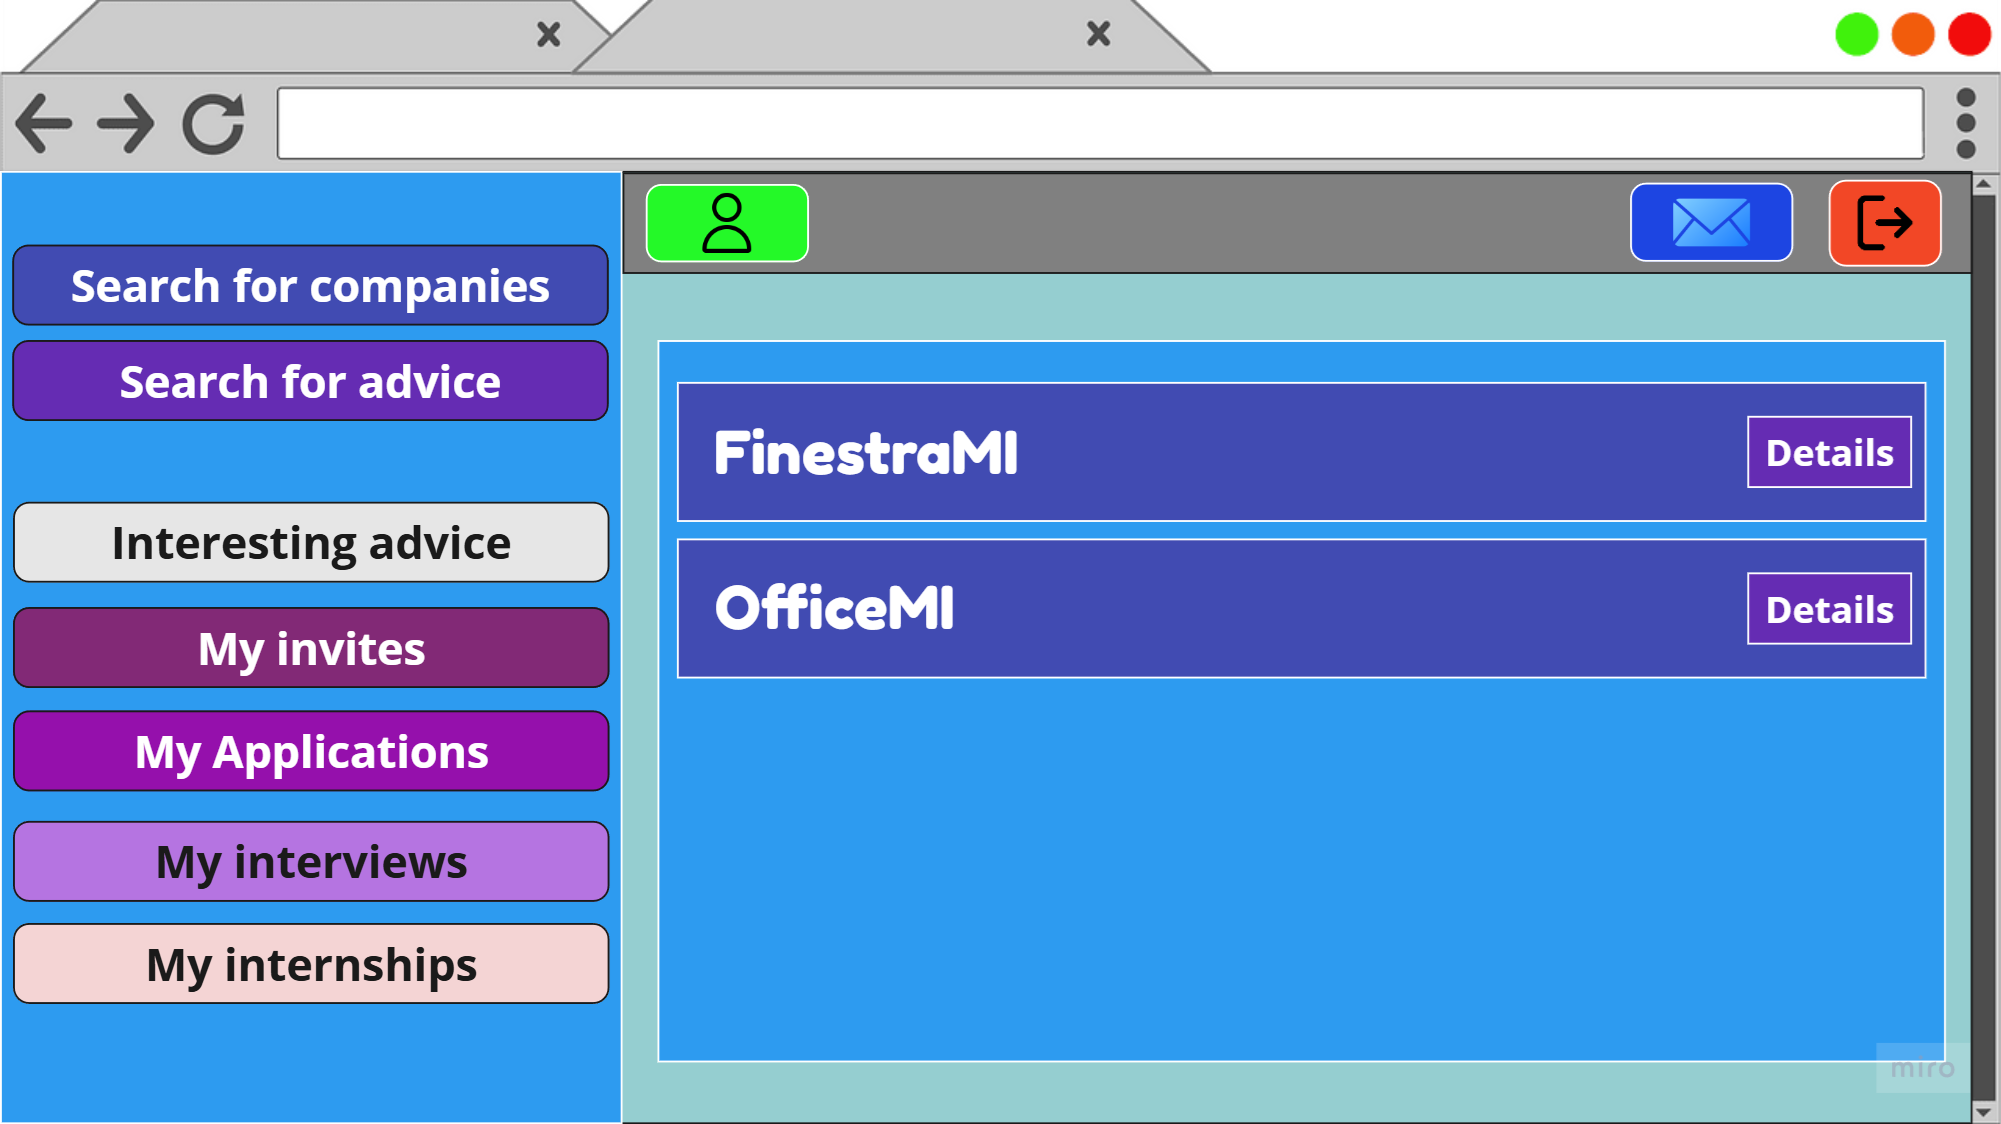
\includegraphics[width=11cm]{UI/interestingInternships.png}
	\end{figure}
	\subsection{Invites and Applications pages}
	\subsubsection{Invites and Applications pages mock-up}
	\begin{figure}[H]
		\centering
		\caption{InvitesPage and ApplicationsPage mock-up}
		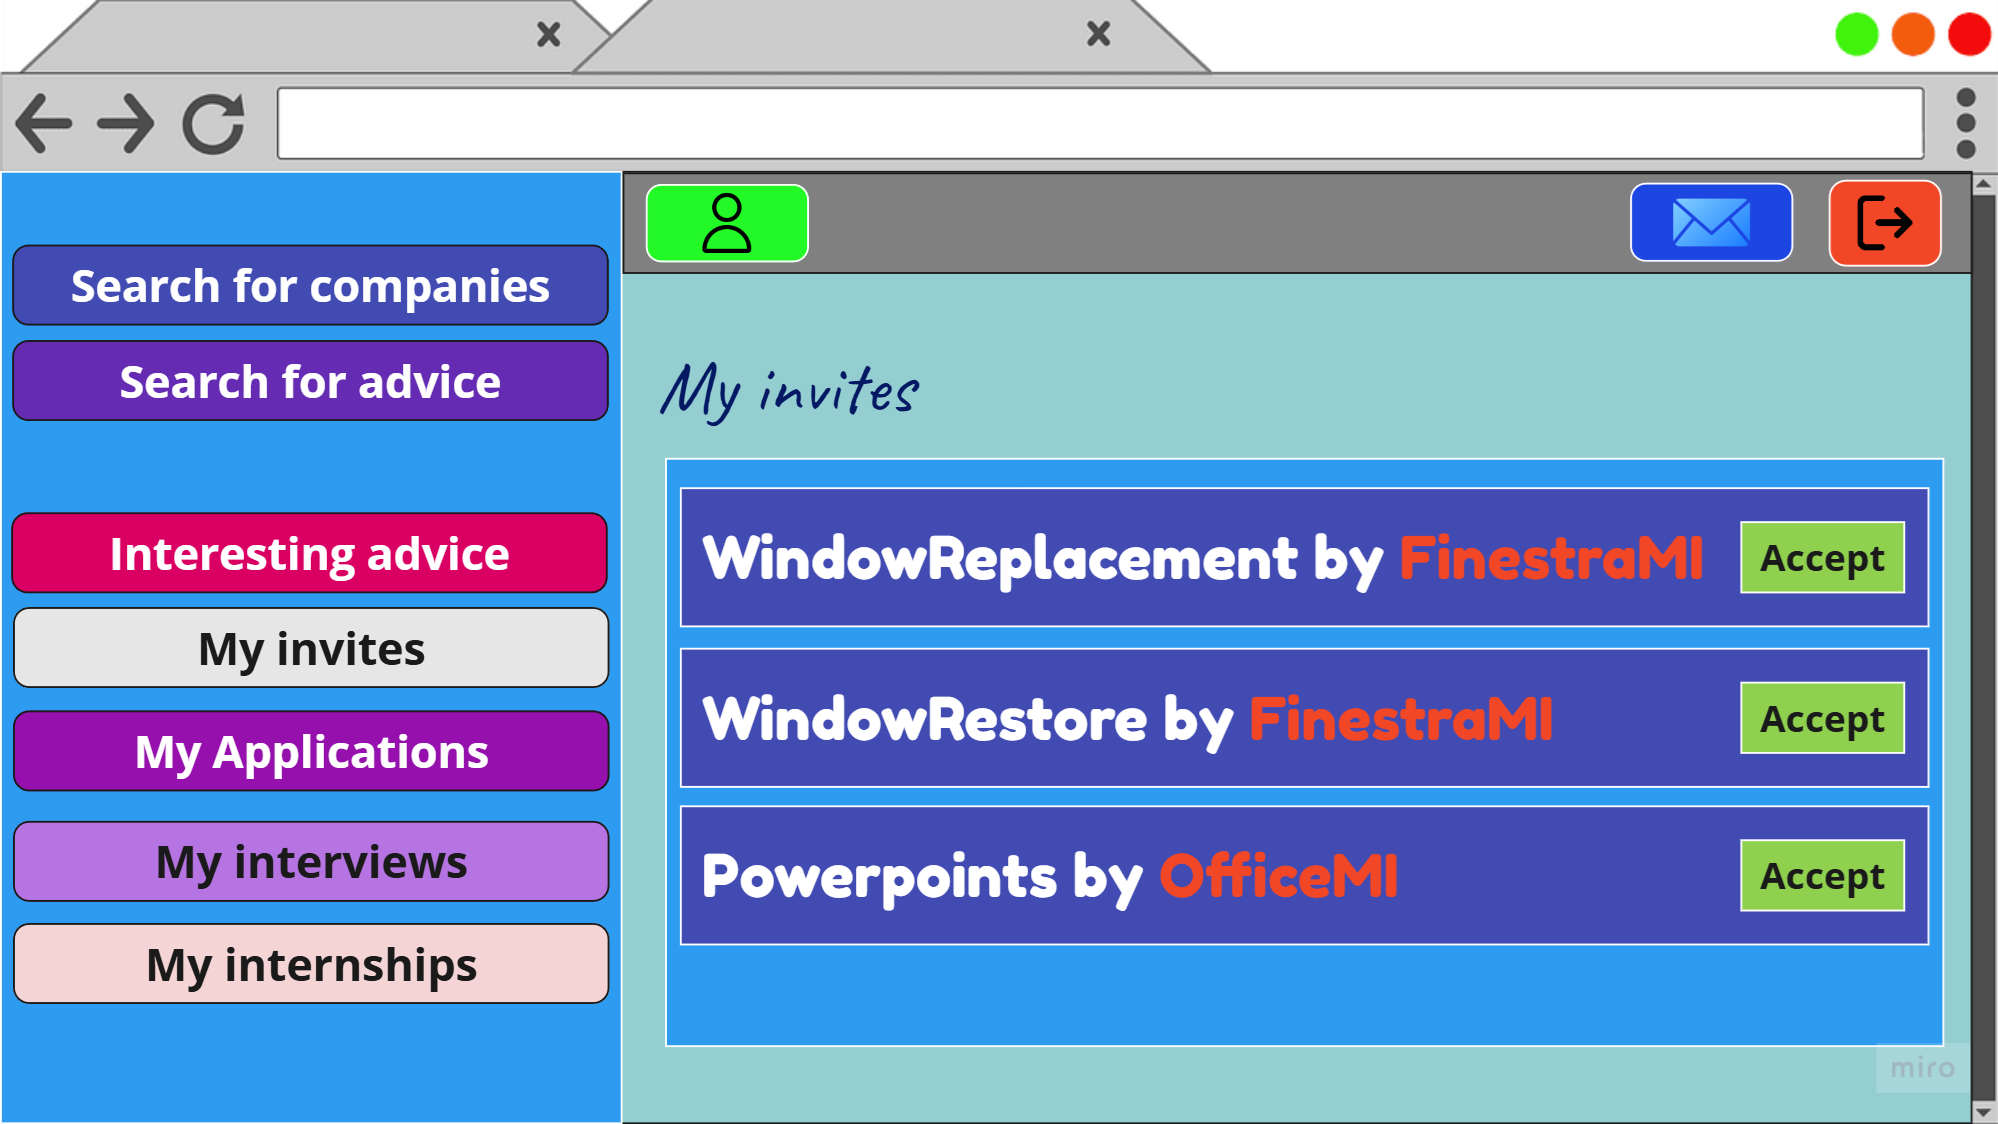
\includegraphics[width=14cm]{UI/invitesApplications.png}
	\end{figure}
	\subsection{Process-related pages}
	\subsubsection{Process-related pages mock-up}
	\begin{figure}[H]
		\centering
		\caption{ConfigProcessPage mock-up}
		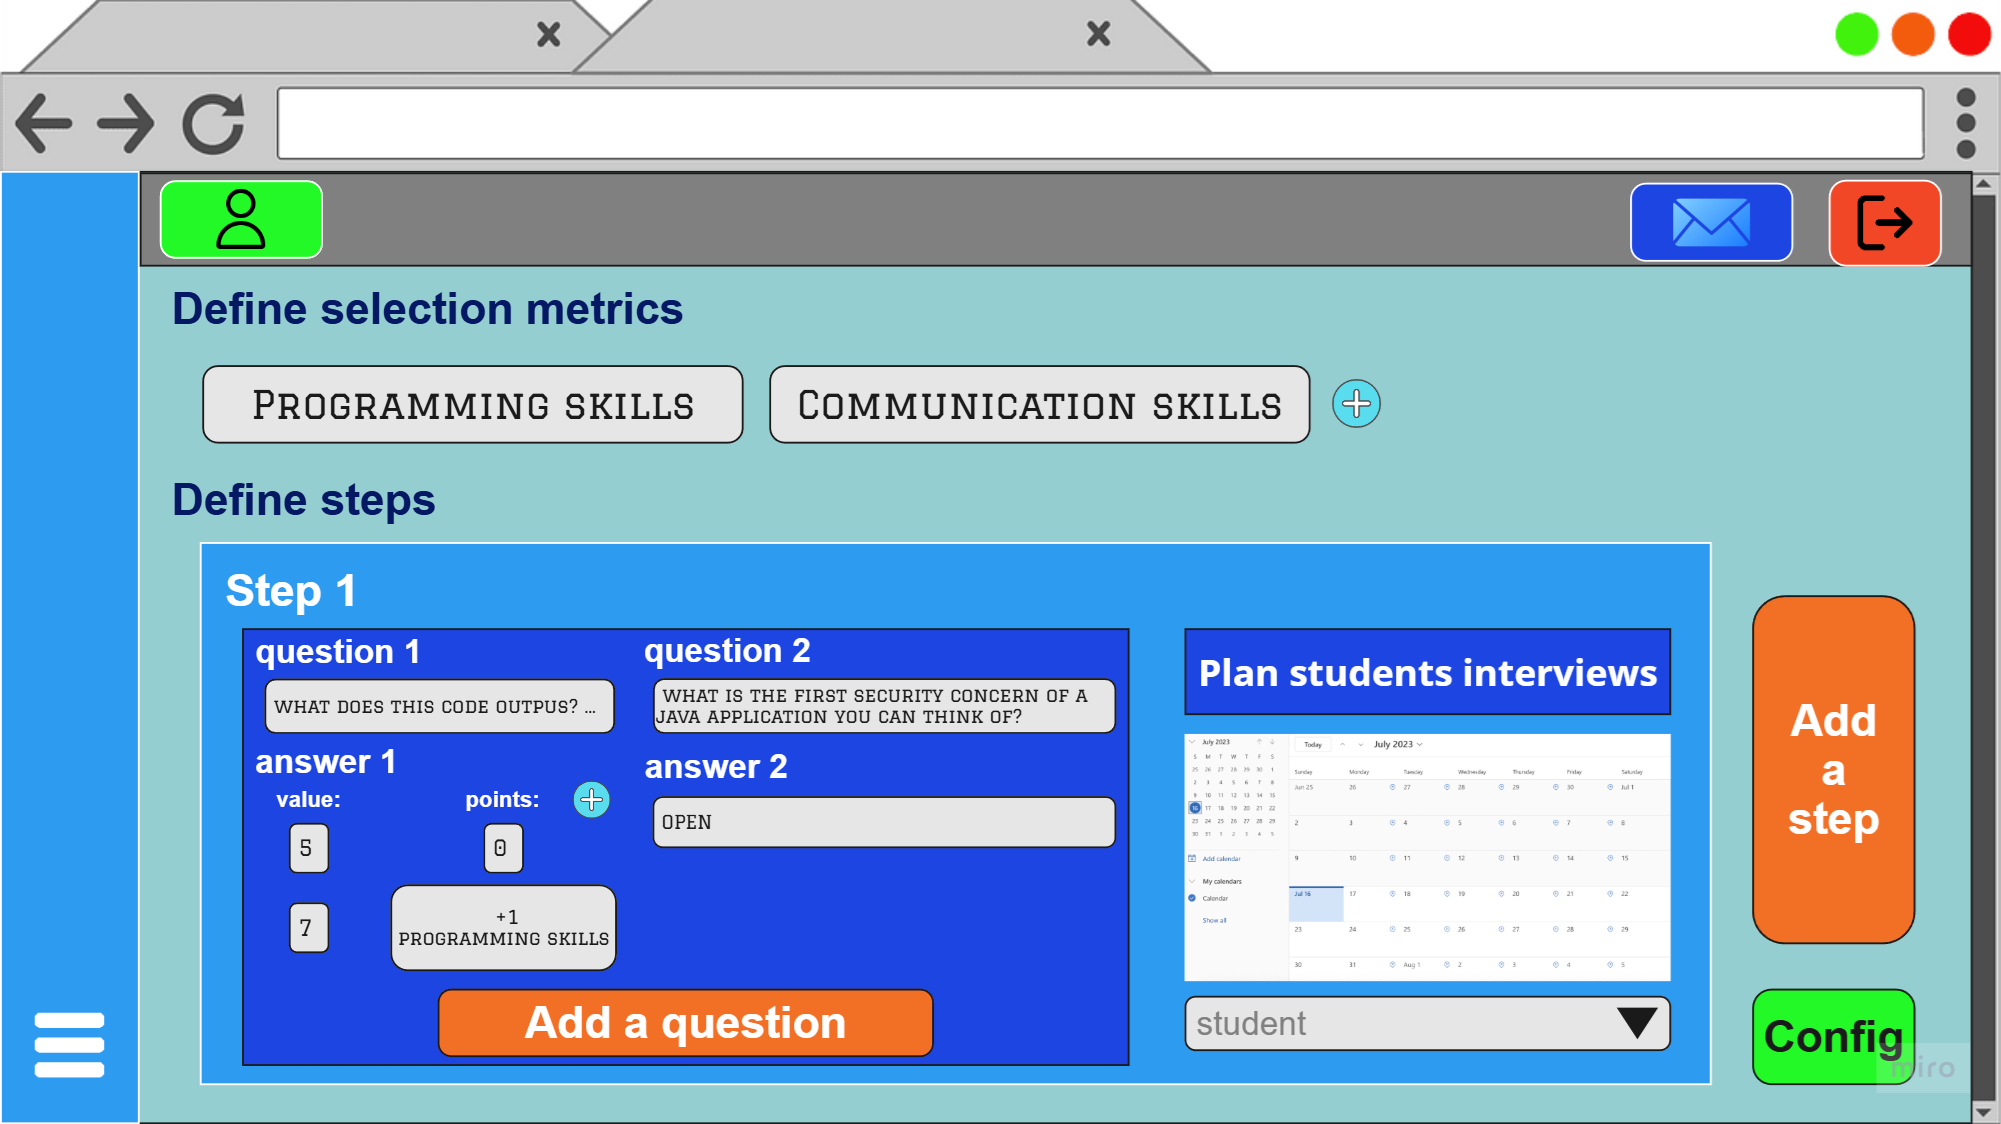
\includegraphics[width=11cm]{UI/configProcess.png}
	\end{figure}
	\begin{figure}[H]
		\centering
		\caption{ProcessManagementPage, StepsManagementPage, ViewStatsPage and ProcessFinalizationPage mock-up}
		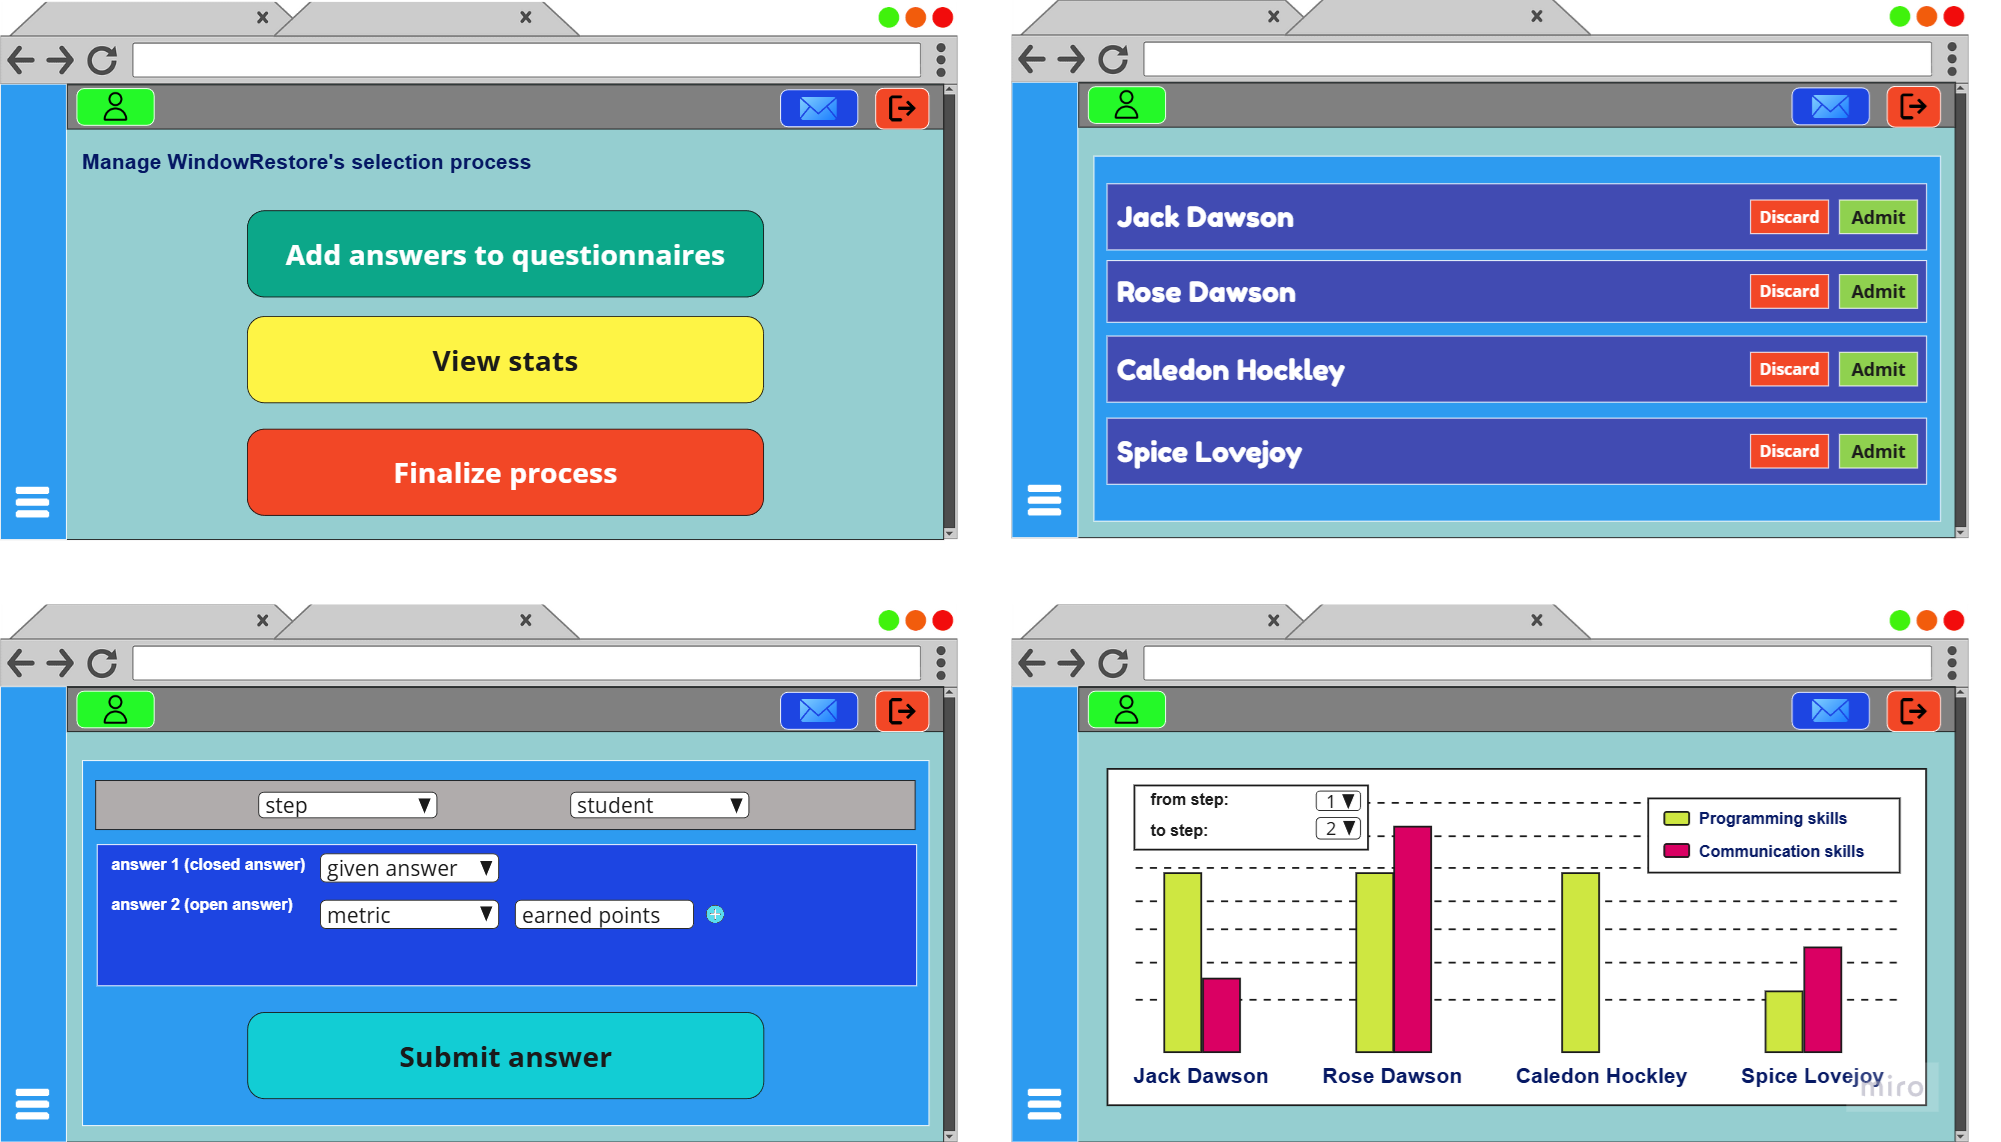
\includegraphics[width=15cm]{UI/viewProcess.png}
	\end{figure}
	\subsection{Interviews pages}
	\subsubsection{Interviews pages mock-up}
	\begin{figure}[H]
		\centering
		\caption{InterviewsPage mock-up}
		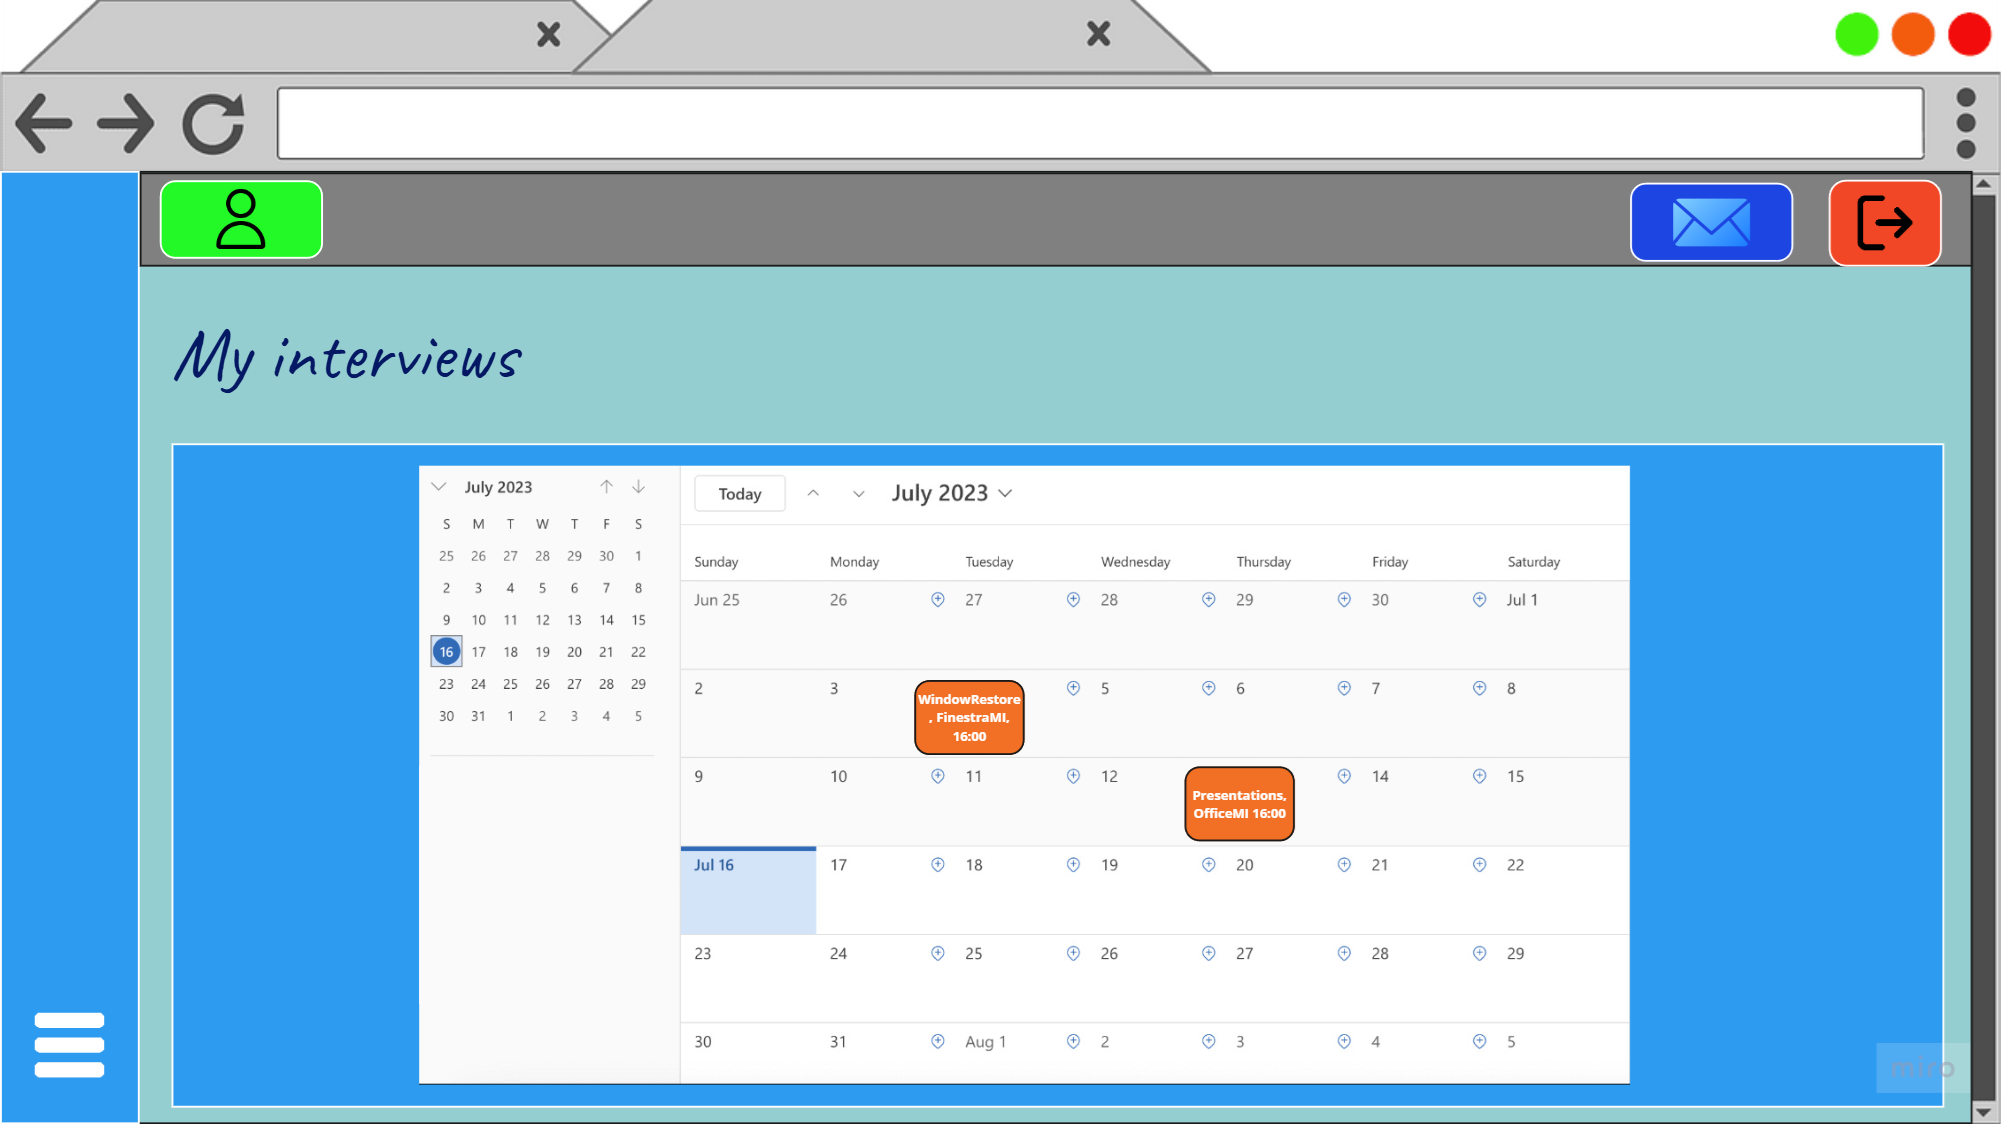
\includegraphics[width=15cm]{UI/myInterviews.png}
	\end{figure}
	\subsection{Internships pages}
	\subsubsection{Internships pages mock-up}
	\begin{figure}[H]
		\centering
		\caption{InternshipsPage and InternshipDetailsPage mock-up (from students view point)}
		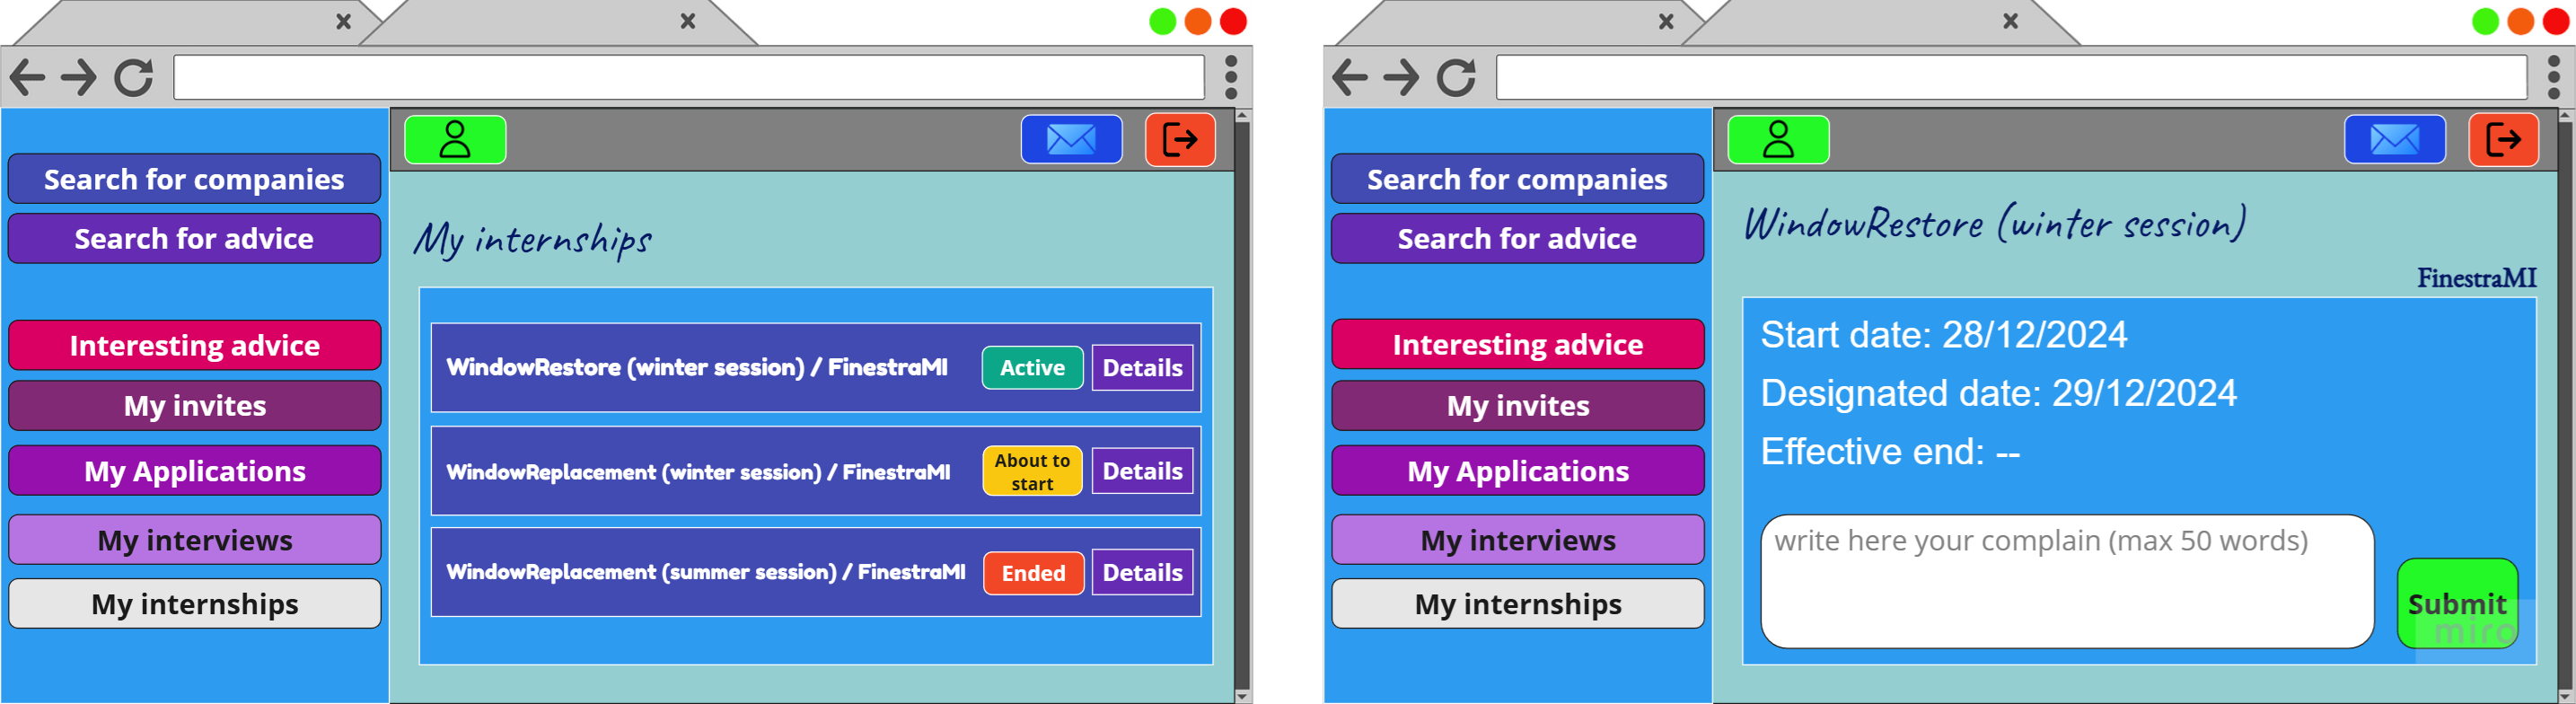
\includegraphics{UI/ongoingPage.png}
	\end{figure}
	In fact there is not much difference in what internships owners see. Companies can end instantly any ongoing internship that belongs to them.
	\section{Requirements UI sections mapping}
		\begin{table}[H]
			\begin{tabular}{ | m{6cm} | m{6cm} | } 
				\hline
					\textbf {RASD UI section} & \textbf{DD pages} \\
				\hline
					registration & WelcomePage, RegistrationMenuPage, StudentRegistrationPage, CompanyRegistrationPage\\
				\hline
					login & LoginPage\\
				\hline
					profiles & StudentProfilePage, CompanyProfilePage \\
				\hline
					notifications & NotificationsPage\\
				\hline
					internship (of a company) & PersonalAdvicePage\\
				\hline
					ongoing & InternshipsPage, InternshipDetailsPage\\
				\hline
					view internships & AdviceSearchPage\\
				\hline
					view companies & CompanySearchPage\\
				\hline
					interesting internships & InterestingAdvicePage\\
				\hline
					invites section & InvitesPage\\
				\hline
					publish new internship & PublishAdvicePage\\
				\hline
					selection process management & ConfigProcessPage, ProcessManagementPage, StepsManagementPage, ViewStatsPage, ProcessFinalizationPage \\
				\hline
			\end{tabular}
			\caption{Requirements UI sections mapping}
		\end{table}